\section{Linearization}\label{se:linearization}
%To be able to obtain a MPC control algorithm the system needs to be transform into state space form. In this section it will be elaborated how this is obtained.
The linearization of the setup can be split into two parts, the first being linearization of pipes and the second of tanks. 

Linearization of pipes is elaborated in the following.
If the simulation environment should be setup with a real sewer system it would be ideal to have a linear model which could mimic a real world situation.
In real systems measurements from all states, which in this case is flow and height in the amount of sections each pipe consists of, is rarely available.
In these cases states are often estimated by an observer or a Kalman filter. By the assumption that height measurements are a more obtainable solution, due to the hostile environment, which sewers typically consists of, it is decided to proceed with a linearized model where the states represent fluid height.

The continuity equation from section \ref{se:hydraulics_of_sewer_line}, and the equation that describes flow in a pipe knowing the height, is used. 
\begin{equation}\label{eq:linearization_Continuity}
\frac{\partial A(x,t)}{\partial t} + \frac{\partial Q(x,t)}{\partial x}=0
\end{equation}

\begin{equation}\label{eq:flow_eq_given_a_height}
	Q = f(h) = \left(0.46-0.5 \cdot cos\left(\pi \frac{h}{d}\right)+0.04\cdot cos\left(2\pi\frac{h}{d}\right)\right)Q_f
\end{equation}

%To be able to implement control in this project, some form of measurement is needed from the pipe. Because it is needed to get information about the condition in the pipe to be able to control it. Therefore it is assumed that it is possible to measure the height of the wastewater in the pipe.

%\fxnote{Ved ikke om det skal stå her (det skal det vist ikke). Somewhere in the report you need to put some words on how you get information above x(k|k). If you should measure it, it means that you should have level measurements along the pipe which is a bit realistic. Therefore, ideas to avoid this must be described somewhere (though you don't need to build a method.)} 

%In the state space model it is desired to have the states as heights of the wastewater. Therefore, equation \ref{eq:linearization_Continuity}, is expanded to the following:
First the continuity equations is expanded to the following:
\begin{equation}
	\frac{\partial A(h)}{\partial h}\frac{\partial h(x,t)}{\partial t} + \frac{\partial Q(h)}{\partial h}\frac{\partial h(x,t)}{\partial x}=0
\end{equation}

By applying equation \ref{eq:preissmann_time_derivatie} and \ref{eq:preissmann_space_derivatie}, from the Preissmann scheme in section \ref{se:preissmann_scheme}, on the partial derivate of h in terms of time and position, the following is obtained: 

\begin{equation}\label{eq:preissmann_skrevet_om}
\begin{aligned}
	&\frac{\partial A(h)}{\partial h} \left(\frac{1}{2}\frac{h_{j+1}^{i+1}-h_{j+1}^i}{\Delta t} +  \frac{1}{2} \frac{h_{j}^{i+1} - h_j^i}{\Delta t}\right) + \\ &\frac{\partial Q(h)}{\partial h}\left(\theta \frac{h_{j+1}^{i+1}-h_j^{i+1}}{\Delta x}+(1-\theta)\frac{h_{j+1}^i - h_j^i}{\Delta x}\right)=0
\end{aligned}
\end{equation}
Where the derivate of Q given h can be found by taking the derivate of equation \ref{eq:flow_eq_given_a_height} with respect to h, and the derivate of A can be found by taking the derivate of the following equation with respect to h:
\begin{equation}%\label{eq:calc_area_open_channel}
	A = \frac {d^2}{4} \cdot acos \left(\frac{\frac{d}{2}-h}{\frac{d}{2}}\right)-\sqrt{h\cdot (d-h)}\cdot  \left(\frac{d}{2}-h\right)
\end{equation}

Setting equation \ref{eq:preissmann_skrevet_om} onto matrix form yields the following:

\begin{equation}\label{eq:rearrange_continuity_eq}
\begin{aligned}
	&\begin{bmatrix}
		\underbrace{\frac{1}{2\Delta t}\frac{\partial A}{\partial h}-\frac{\theta}{\Delta x}\frac{\partial Q}{\partial h}}_{a} & \underbrace{\frac{1}{2\Delta t}\frac{\partial A}{\partial h}+\frac{\theta}{\Delta x}\frac{\partial Q}{\partial h}}_{b} 
	\end{bmatrix}
	\begin{bmatrix}
		h_{j}^{i+1} \\
		h_{j+1}^{i+1}
	\end{bmatrix}
	= \\ -
	&\begin{bmatrix}
		\underbrace{\frac{-1}{2\Delta t}\frac{\partial A}{\partial h}-\frac{(1-\theta)}{\Delta x}\frac{\partial Q}{\partial h}}_{c} & \underbrace{\frac{-1}{2\Delta t}\frac{\partial A}{\partial h}+\frac{\theta}{\Delta x}\frac{\partial Q}{\partial h}}_{d} 
	\end{bmatrix}
	\begin{bmatrix}
		h_{j}^{i} \\
		h_{j+1}^{i}
	\end{bmatrix}
	\end{aligned}
\end{equation}

This equation can be written on state space form, where the heights are the states of the state space system and a, b, c, and d are the parameters in the system matrix and the input vector. %As the equations are discretized a discretized state space model is needed: 

\begin{equation}
	x(k+1) = Ax(k) + Bu(k) + B_dd(k)
\end{equation}
Where A is the system matrix, x is the states of the system, B is the input vector, u is the input, $B_d$ is the input disturbance vector and d is the disturbance input. By utilizing equation \ref{eq:rearrange_continuity_eq} the following can be written:

\begin{equation}
\begin{aligned}
	   \underbrace{\begin{bmatrix}
	    	1 & 0    & 0    &\cdots &0\\
	    	0 & b_1  & 0    &\cdots &0\\
	    	0 &a_{1} & b_2  &\cdots &\vdots	  \\
	    \vdots&\vdots&\ddots&\ddots & 0  \\
	        0 & 0    &0  	&a_{m-1}&  b_m\\
	   \end{bmatrix}}_{\xi}
	    \underbrace{\begin{bmatrix}
		h_{0}^{i+1}\\
		h_{1}^{i+1} \\
		h_{2}^{i+1} \\			
		\vdots		\\
		h_{m}^{i+1}\\
	\end{bmatrix}}_{x(k+1)}
	=& 
	\underbrace{\begin{bmatrix}
	    	0 &  0   &   0    & \cdots   &0\\
	    c_{0} & d_1  &   0    &  \cdots  &0\\
	    0	  &c_{1} & d_2    & \cdots   &0 \\
	    \vdots&\vdots&\ddots  & \ddots   & \vdots\\
	    0	  & 0    &  0     &  c_{m-1} &  d_m\\
	    \end{bmatrix}}_{A}
	    	\underbrace{\begin{bmatrix}
		h_{0}^{i} \\
		h_{1}^{i} \\
		h_{2}^{i}\\
		\vdots		\\
		h_{m}^{i}\\
		\end{bmatrix}}_{x(k)}
	+ \\ & \underbrace{\begin{bmatrix}
		 1\\
		 -a_0 \\
		 0\\
		 \vdots \\
		 0\\
		\end{bmatrix}}_{B}
		h_0^{i+1}
		% \underbrace{\begin{bmatrix}
		% h_{0}^{i} \\
		% h_{0}^{i+1} \\
		% \end{bmatrix}}_{u}
		+ 
		\underbrace{\begin{bmatrix}
		 \frac{dh}{dQ}\\
		 0 \\
		 0\\
		 \vdots \\
		 0\\
		\end{bmatrix}}_{B_d}
		d_{0}^{i+1}
	\end{aligned}
\end{equation}
Where m denotes the total amount of sections in the pipe.  
To obtain a state space form $\xi$ needs to inversed, thereby obtaining the following equation:

\begin{equation}
	x(k+1) = \xi^{-1} (Ax(k)+Bu(k)+B_dd(k))
\end{equation}

By repeating this procedure the desired amount of pipes can be inserted into the linear model. Due to equation \ref{eq:rearrange_continuity_eq} containing discretizing elements in the form of $\Delta t$ and $\Delta x$ no discretizing of the state space system should be necessary. A verification in the form of a comparison of the nonlinear and linear system is performed further on. 

The change of height within the tank is given by $h = Q_{in}-Q_{out}$.

As the input to the tank is a height in an adjoining pipe the inflow to the tank needs to be obtained from it. This means that the derivative of h(Q) is needed. As mentioned in section \ref{sec:implementation} equation \ref{eq:flow_eq_given_a_height} can not be solved for h analytically. Instead a curve fitted polynomial is created for the inflowing pipe and the derivative is obtained by the MATLAB function ``differentiate''. The increase in height within the tank by the inflow is given by:
\begin{equation} \label{eq:heigh_in_flow_lin_tank}
	h_{inflow} = h_{pipe} \cdot \frac{dh}{dQ} \cdot \frac{1}{A} \cdot \Delta t 
\end{equation}
Where $h_{pipe}$ is the inflow height in the adjoining pipe and A is the vertical cross section area of the tank.

The outflow of the tank is due to being controlled by the pump split into two parts. The first being the change in height within the tank due to the pump, and secondly the height into the adjoining pipe due to the outflow controlled by the pump. 
As seen in equation \ref{eq:final_pump_model} the outflow of the tank is already a linear term, therefore the reduction in height due to the pump is:
\begin{equation}\label{eq:height_reduc_pump_lin_tank}
 	h_{pump} = u_{pump} \cdot Q_{max\_out} \cdot \Delta t
\end{equation} 

The change of height is then given by:
\begin{equation}
	h_{tank} = h_{inflow} - h_{pump}
\end{equation}

Finally the inflow to the adjoining pipe is given by:
\begin{equation} \label{eq:height_outflow_lin_tank}
	h_{outflow} = \frac{dQ}{dh} \cdot u_{pump} \cdot Q_{max\_out}
\end{equation}
Where the derivative is found by curve fitted polynomial and the MATLAB function ``differentiate''.
Utilizing the same indexing scheme on equation \ref{eq:heigh_in_flow_lin_tank}, \ref{eq:height_reduc_pump_lin_tank} and \ref {eq:height_outflow_lin_tank} as in equation \ref{eq:rearrange_continuity_eq} the following is given:


	$\underbrace{\frac{dh}{dQ} \cdot \frac{1}{A} \cdot \Delta t}_{e}$ , $\underbrace{u_{pump} \cdot Q_{max\_out} \cdot \Delta t}_{f}$, $\underbrace{\frac{dQ}{dh} \cdot u_{pump} \cdot Q_{max\_out}}_{g}$ 
\\
An example of how the tank is implemented in a state space system in between two pipes, can be seen in equation \ref{eq:tank_linear_implement_ss}

\begin{equation}\label{eq:tank_linear_implement_ss}
\begin{aligned}
      & \underbrace{\begin{bmatrix}
            1 & 0       & 0         &0          &0          &0   &0\\
            0 & b_{1,1} & 0         &0          &0          &0  &0\\
            0 &a_{1,1}  & b_{1,2}   & 0         &0          &0 &0\\
            0 &0        & 0         & 1         & 0         &0      &0\\
             0 &0        & 0         &  0        & 1         &0   & 0        \\
            0 & 0       &0          &  0         &a_{2,1}    &  b_{2,2}&0       \\
            0 & 0       & 0         &   0        &     0      & a_{2,2}  & b_{2,3}\\  
       \end{bmatrix}}_{\xi}
        \underbrace{\begin{bmatrix}
        h_{1,0}^{i+1}\\
        h_{1,1}^{i+1} \\
        h_{1,2}^{i+1} \\ 
        h_{tank}^{i+1} \\          
        h_{2,0}^{i+1}     \\
        h_{2,1}^{i+1}\\
    \end{bmatrix}}_{x(k+1)}
    \\ &=
    \underbrace{\begin{bmatrix}
        0       &  0    &   0    & 0     &0         &0          &0 \\
        c_{1,0} &d_{1,1}&   0    &  0    &0         &0          &0\\
        0       &c_{1,1}& d_{1,2}& 0     &0         &0       &0\\
        0       & 0     & e    & 1     &0         &0          &0           \\
        0       & 0     &   0    & 0     & 0        &0          &0        \\
        0       & 0     &  0     & 0    &c_{2,0}    &  d_{2,1} &0  \\
         0       & 0     &  0    & 0    &0          &c_{2,1}    &  d_{2,2}   \\
        \end{bmatrix}}_{A}
            \underbrace{\begin{bmatrix}
        h_{1,0}^{i} \\
        h_{1,1}^{i} \\
        h_{1,2}^{i} \\
        h_{tank}^{i}\\
        h_{2,0}^{i}\\
        h_{2,1}^{i}\\
          h_{2,2}^{i}\\
        \end{bmatrix}}_{x(k)}
    +  \underbrace{\begin{bmatrix}
         1 & 0\\
         -a_0& 0 \\
         0 & 0\\
          0& -f \\
          0& g \\ 
          0& 0 \\
          0& 0 \\
        \end{bmatrix}}_{B}
        \begin{bmatrix}
        h_0^{i+1}\\
        u_{tank} \\
        \end{bmatrix}
    \end{aligned}
\end{equation}

Where subscripts indicate pipe and section number.

A test of the linear system has been conducted to verify if the linear model has a similar response of the nonlinear model for small perturbations. %Therefore, a test has been conducted on the sewer network setup where the specification for the pipes are shown in figure \ref{fig:Fredericia_pipe_setup} and the specification for the tank placed after the first pipe is seen in \ref{tab:tank_data_nonlinear_linear_test} 
In table \ref{tab:system_setup_nonlinear_linear_test} the system setup which is used to verify the linear model is seen.

\begin{table}[H]
\centering
\begin{tabular}{|c|c|c|}
\hline
	\rowcolor[HTML]{9B9B9B} 
Type  & Components & Sections \\ \hline
Pipe  & 1         & 35       \\ \hline
Tank  & 1         & 1        \\ \hline
Pipe  & 18        & 227      \\ \hline
Total & 20        & 263      \\ \hline
\end{tabular}
\caption{System setup for verification of linear model.}
\label{tab:system_setup_nonlinear_linear_test}
\end{table}

What is important to remember before simulating is that the state space system is a small signal model. This is also the reason why the nonlinear systems needs to be brought into steady state before the linearized model is obtained. If the system is not in steady state the linearized model is most likely going to yield an undesirable result. 
The first part shown in table \ref{tab:system_setup_nonlinear_linear_test} has the specifications seen in table \ref{tab:pipe_data_nonlinear_linear_test}.

\begin{table}[H]
\centering
\begin{tabular}{|c|c|c|c|c|c|c|c|}
\hline
\rowcolor[HTML]{9B9B9B} 
\begin{tabular}[c]{@{}c@{}}Part\\ number\end{tabular} & Length {[}m{]} & Sections & Dx {[}m{]} & Sb     & d {[}m{]} & $\theta$ & $Q_f $  {[}$m^3/s${]} \\ \hline
1                                                          & 700            & 35       & 20         & 0,003  & 0,9       & 0,65     & 0,972                                                                          \\ \hline
\end{tabular}
\caption{Specification of the first pipe in the comparison of the nonlinear with the linear model.}
\label{tab:pipe_data_nonlinear_linear_test}
\end{table}

Pipe specifications for the remaining 18 pipes can be seen in figure \ref{fig:Fredericia_pipe_setup}. In table \ref{tab:tank_data_nonlinear_linear_test} specifications of the tank can be seen.



% \begin{table}[H]
% \centering
% \begin{tabular}{|c|c|c|c|c|c|c|c|}
% \hline
% \begin{tabular}[c]{@{}c@{}}Component\\ number\end{tabular} & Length {[}m{]} & Sections & Dx {[}m{]} & Sb     & d {[}m{]} & $\theta$ & \begin{tabular}[c]{@{}c@{}}$Q_f $\\  {[}$m^3/s${]}\end{tabular} \\ \hline
% 1                                                          & 700            & 35       & 20         & 0,003  & 0,9       & 0,65     & 0,972                                                                          \\ \hline
% 3                                                          & 303            & 15       & 20,2       & 0,003  & 0,9       & 0,65     & 0,972                                                                          \\ \hline
% 4                                                          & 27             & 1        & 27         & 0,003  & 1         & 0,65     & 1,284                                                                          \\ \hline
% 5                                                          & 155            & 8        & 19,4       & 0,0041 & 1         & 0,65     & 1,50                                                                           \\ \hline
% 6                                                          & 295            & 14       & 21         & 0,0122 & 0,8       & 0,65     & 1,438                                                                          \\ \hline
% 7                                                          & 318            & 15       & 21,2       & 0,0053 & 0,9       & 0,65     & 1,293                                                                          \\ \hline
% 8                                                          & 110            & 5        & 22         & 0,0036 & 0,9       & 0,65     & 1,066                                                                          \\ \hline
% 9                                                          & 38             & 2        & 19         & 0,0024 & 1         & 0,65     & 1,149                                                                          \\ \hline
% 10                                                         & 665            & 30       & 22,2       & 0,003  & 1         & 0,65     & 1,284                                                                          \\ \hline
% 11                                                         & 155            & 7        & 22,1       & 0,0008 & 1         & 0,65     & 0,663                                                                          \\ \hline
% 12                                                         & 955            & 40       & 23,9       & 0,0029 & 1,2       & 0,65     & 2,041                                                                          \\ \hline
% 13                                                         & 304            & 15       & 20,3       & 0,003  & 1,2       & 0,65     & 2,076                                                                          \\ \hline
% 14                                                         & 116            & 5        & 23,2       & 0,0021 & 1,2       & 0,65     & 1,737                                                                          \\ \hline
% 15                                                         & 283            & 12       & 23,6       & 0,0017 & 1,4       & 0,65     & 2,346                                                                          \\ \hline
% 16                                                         & 31             & 1        & 31         & 0,0019 & 1,4       & 0,65     & 2,480                                                                          \\ \hline
% 17                                                         & 125            & 6        & 20,8       & 0,0021 & 1,6       & 0,65     & 3,707                                                                          \\ \hline
% 18                                                         & 94             & 4        & 23,5       & 0,0013 & 1,5       & 0,65     & 2,461                                                                          \\ \hline
% 19                                                         & 360            & 15       & 24         & 0,0046 & 1,6       & 0,65     & 5,487                                                                          \\ \hline
% 20                                                         & 736            & 32       & 23         & 0,0012 & 1,6       & 0,65     & 2,802                                                                          \\ \hline
% \end{tabular}
% \caption{The specification on the pipes for comparing the nonlinear model with the linear model.}
% \label{tab:pipe_data_nonlinear_linear_test}
% \end{table}


\begin{table}[H]
\centering
\begin{tabular}{|c|c|}
\hline
Part number& 2 (Tank)  \\ \hline
Size $[m^3]$                                              & 90 \\ \hline
Height {[}m{]}                                             & 10 \\ \hline
Area {[}$m^2$                                              & 9  \\ \hline
\end{tabular}
\caption{Tank specification of the tank used in comparison of the nonlinear model with the linear. }
\label{tab:tank_data_nonlinear_linear_test}
\end{table}



% It can be seen that the setup consist of 19 pipes and one tank. The input to the pipes after tank is a sinus wave as is shown in figure \ref{fig:height_input_for_comparision}.  

% \begin{figure}[H]
%  \centering
%  % This file was created by matlab2tikz.
%
%The latest updates can be retrieved from
%  http://www.mathworks.com/matlabcentral/fileexchange/22022-matlab2tikz-matlab2tikz
%where you can also make suggestions and rate matlab2tikz.
%
\definecolor{mycolor1}{rgb}{0.00000,0.44700,0.74100}%
%
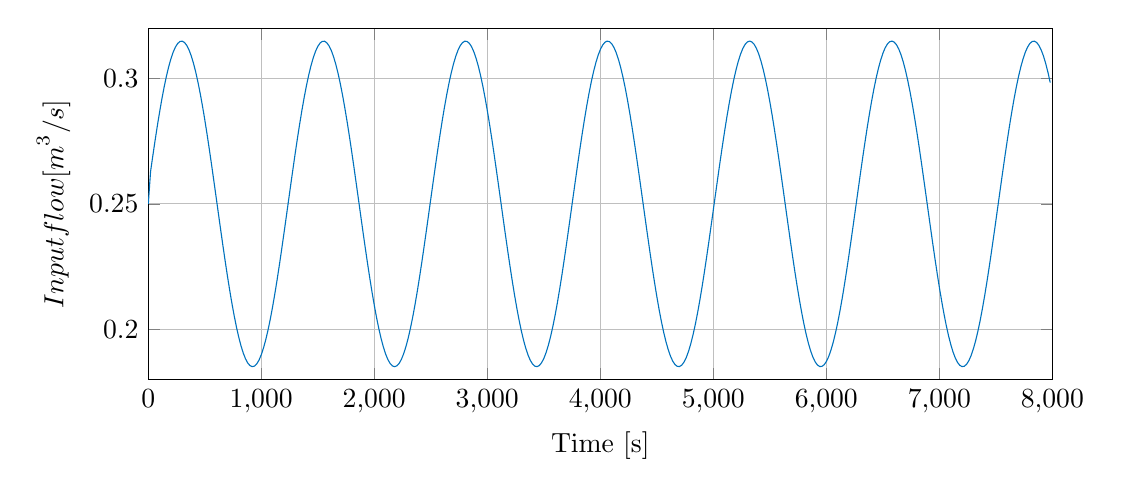
\begin{tikzpicture}

\begin{axis}[%
width=4.521in,
height=1.7566in,
at={(0.758in,0.481in)},
scale only axis,
xmin=0,
xmax=8000,
xlabel={Time [s]},
xmajorgrids,
ymin=0.18,
ymax=0.32,
ylabel={$\text{Input flow [m}^\text{3}\text{/s]}$},
ymajorgrids,
axis background/.style={fill=white}
]
\addplot [color=mycolor1,solid,forget plot]
  table[row sep=crcr]{%
1	0.250000001997809\\
21	0.262886754653035\\
41	0.269169019141146\\
61	0.275259753146396\\
81	0.281098100067933\\
101	0.286625725073218\\
121	0.291787397960388\\
141	0.296531545000176\\
161	0.300810764243567\\
181	0.304582299146404\\
201	0.307808465778641\\
221	0.310457029349718\\
241	0.31250152628793\\
261	0.313921528655692\\
281	0.314702848258737\\
301	0.314837678409859\\
321	0.314324671930759\\
341	0.313168954612597\\
361	0.311382074000788\\
381	0.308981884015741\\
401	0.305992366562389\\
421	0.302443391910922\\
441	0.298370420242923\\
461	0.293814147344954\\
481	0.288820097989707\\
501	0.283438171067526\\
521	0.27772214101319\\
541	0.271729120509533\\
561	0.265518989836398\\
581	0.259153798566676\\
601	0.25269714558748\\
621	0.246213543641094\\
641	0.239767774734971\\
661	0.233424242861334\\
681	0.227246330493771\\
701	0.221295765290512\\
721	0.215632003332074\\
741	0.210311635055753\\
761	0.205387819822688\\
781	0.20090975476709\\
801	0.196922183234743\\
821	0.193464947722282\\
841	0.190572591784138\\
861	0.188274014884759\\
881	0.186592183644715\\
901	0.185543902365817\\
921	0.185139645128088\\
941	0.185383451136218\\
961	0.186272884361165\\
981	0.187799057880153\\
1001	0.189946722671866\\
1021	0.192694419979629\\
1041	0.19601469572021\\
1061	0.199874374795948\\
1081	0.204234892569357\\
1101	0.209052680188242\\
1121	0.214279599911263\\
1141	0.219863426084337\\
1161	0.225748366962111\\
1181	0.231875622160638\\
1201	0.238183970171374\\
1221	0.244610380066258\\
1241	0.251090641281911\\
1261	0.257560005190354\\
1281	0.263953832045903\\
1301	0.270208236844133\\
1321	0.276260727639734\\
1341	0.282050829945362\\
1361	0.287520690972733\\
1381	0.292615657678558\\
1401	0.297284822839683\\
1421	0.30148153370124\\
1441	0.305163858115549\\
1461	0.308295003514275\\
1481	0.310843684527614\\
1501	0.312784435577363\\
1521	0.31409786532056\\
1541	0.314770850401372\\
1561	0.314796666575332\\
1581	0.314175055895763\\
1601	0.312912229291097\\
1621	0.311020804507335\\
1641	0.308519680035693\\
1661	0.30543384628513\\
1681	0.301794135886441\\
1701	0.297636915622801\\
1721	0.293003723064891\\
1741	0.287940851541218\\
1761	0.282498887590485\\
1781	0.276732205517613\\
1801	0.270698424103663\\
1821	0.26445783089802\\
1841	0.258072779845129\\
1861	0.251607068264493\\
1881	0.245125299408945\\
1901	0.238692236970304\\
1921	0.232372157981967\\
1941	0.226228210584045\\
1961	0.220321783068021\\
1981	0.214711890505228\\
2001	0.20945458508777\\
2021	0.204602396073545\\
2041	0.200203804931261\\
2061	0.196302760929632\\
2081	0.192938242010808\\
2101	0.190143865335664\\
2121	0.18794755139224\\
2141	0.186371245023454\\
2161	0.185430696161485\\
2181	0.185135302459658\\
2201	0.185488015394197\\
2221	0.186485310774052\\
2241	0.188117223953449\\
2261	0.190367449395338\\
2281	0.19321350359093\\
2301	0.196626949707483\\
2321	0.200573681719736\\
2341	0.205014265186038\\
2361	0.209904331264255\\
2381	0.215195020030576\\
2401	0.220833468671715\\
2421	0.226763339672675\\
2441	0.232925383722569\\
2461	0.23925803171415\\
2481	0.245698009921982\\
2501	0.252180972212586\\
2521	0.258642142969737\\
2541	0.265016964311009\\
2561	0.271241741128795\\
2581	0.277254277510769\\
2601	0.282994498180884\\
2621	0.288405048751668\\
2641	0.293431868790308\\
2661	0.298024731972623\\
2681	0.302137747927896\\
2701	0.305729820760282\\
2721	0.308765059665423\\
2741	0.311213137539494\\
2761	0.313049593997605\\
2781	0.314256079773878\\
2801	0.314820540061248\\
2821	0.31473733495911\\
2841	0.314007295825339\\
2861	0.312637716969642\\
2881	0.310642282771222\\
2901	0.308040930948987\\
2921	0.304859653350452\\
2941	0.301130236249792\\
2961	0.296889942749893\\
2981	0.292181140461754\\
3001	0.287050878181313\\
3021	0.281550415793439\\
3041	0.275734712100098\\
3061	0.26966187569018\\
3081	0.263392584337679\\
3101	0.256989478729437\\
3121	0.250516536580106\\
3141	0.244038433387972\\
3161	0.237619896218756\\
3181	0.231325056974165\\
3201	0.225216811607134\\
3221	0.219356191686253\\
3241	0.213801754588509\\
3261	0.208608998413328\\
3281	0.203829807463917\\
3301	0.199511933836451\\
3321	0.195698520296917\\
3341	0.192427669212855\\
3361	0.189732061847097\\
3381	0.187638631817393\\
3401	0.186168295984603\\
3421	0.18533574545834\\
3441	0.185149298808259\\
3461	0.185610818947655\\
3481	0.186715694519854\\
3501	0.188452885973362\\
3521	0.190805035865415\\
3541	0.193748642291808\\
3561	0.197254293710156\\
3581	0.201286962810301\\
3601	0.205806356495619\\
3621	0.210767318478317\\
3641	0.21612028046614\\
3661	0.221811757432362\\
3681	0.227784882020486\\
3701	0.233979972744082\\
3721	0.240335130304463\\
3741	0.246786856068022\\
3761	0.253270686523587\\
3781	0.259721837380514\\
3801	0.26607585087191\\
3821	0.272269239795324\\
3841	0.278240121855897\\
3861	0.28392883797379\\
3881	0.289278548377994\\
3901	0.294235800530528\\
3921	0.298751063206534\\
3941	0.3027792213939\\
3961	0.306280027067552\\
3981	0.309218501334409\\
4001	0.311565283930928\\
4021	0.313296926581148\\
4041	0.314396127284113\\
4061	0.314851903189745\\
4081	0.314659700335857\\
4101	0.313821439149829\\
4121	0.312345495260341\\
4141	0.310246615810853\\
4161	0.307545772111028\\
4181	0.304269950098335\\
4201	0.300451880703481\\
4221	0.296129712813773\\
4241	0.291346632102048\\
4261	0.286150429529699\\
4281	0.280593023835195\\
4301	0.2747299427792\\
4321	0.268619768329549\\
4341	0.262323551329587\\
4361	0.255904201498327\\
4381	0.249425858857326\\
4401	0.242953252864798\\
4421	0.236551055660262\\
4441	0.230283235881899\\
4461	0.224212419513071\\
4481	0.218399264144189\\
4501	0.212901852902125\\
4521	0.207775114102807\\
4541	0.203070272425644\\
4561	0.19883433709346\\
4581	0.19510963217188\\
4601	0.191933373681257\\
4621	0.189337297746497\\
4641	0.187347343500193\\
4661	0.185983393907381\\
4681	0.185259077101532\\
4701	0.185181630216741\\
4721	0.185751827076682\\
4741	0.186963970462812\\
4761	0.188805949039098\\
4781	0.191259358364483\\
4801	0.194299684783977\\
4821	0.197896550360995\\
4841	0.202014016403656\\
4861	0.206610942552316\\
4881	0.211641397840439\\
4901	0.217055119621635\\
4921	0.222798015777402\\
4941	0.228812705187703\\
4961	0.235039091064141\\
4981	0.241414961417209\\
5001	0.247876610657921\\
5021	0.254359476123001\\
5041	0.260798783163673\\
5061	0.267130192352538\\
5081	0.273290442341866\\
5101	0.279217981950073\\
5121	0.284853585160777\\
5141	0.290140942889579\\
5161	0.295027225605822\\
5181	0.299463611187795\\
5201	0.303405772737236\\
5221	0.30681432147905\\
5241	0.309655200320925\\
5261	0.311900024140542\\
5281	0.313526363400335\\
5301	0.314517968256018\\
5321	0.314864930919653\\
5341	0.314563784654995\\
5361	0.313617538415976\\
5381	0.312035646782229\\
5401	0.309833915492053\\
5421	0.307034343516705\\
5441	0.303664903253947\\
5461	0.299759261037095\\
5481	0.295356440752147\\
5501	0.290500433924011\\
5521	0.285239760167731\\
5541	0.279626982396533\\
5561	0.273718181630568\\
5581	0.267572396653901\\
5601	0.261251034118491\\
5621	0.254817254989228\\
5641	0.248335343460447\\
5661	0.241870064649509\\
5681	0.235486017485154\\
5701	0.229246989256365\\
5721	0.223215318270854\\
5741	0.217451270991304\\
5761	0.21201243987279\\
5781	0.206953167918012\\
5801	0.202324005699967\\
5821	0.198171206277341\\
5841	0.194536263049232\\
5861	0.191455495166822\\
5881	0.188959684644427\\
5901	0.187073768795781\\
5921	0.185816591068641\\
5941	0.185200712767292\\
5961	0.185232287544136\\
5981	0.185910999914442\\
6001	0.187230068408557\\
6021	0.189176313330114\\
6041	0.191730288443201\\
6061	0.194866475272719\\
6081	0.198553538076553\\
6101	0.202754636941948\\
6121	0.20742779587774\\
6141	0.212526322224584\\
6161	0.21799927319257\\
6181	0.223791964864743\\
6201	0.229846518580725\\
6221	0.236102439241154\\
6241	0.242497219754725\\
6261	0.248966965588378\\
6281	0.255447033180357\\
6301	0.26187267583731\\
6321	0.268179690661843\\
6341	0.274305060046651\\
6361	0.280187581325618\\
6381	0.28576847829063\\
6401	0.290991988464009\\
6421	0.295805920258768\\
6441	0.300162174459687\\
6461	0.304017224814776\\
6481	0.307332552935198\\
6501	0.310075033158275\\
6521	0.312217263528162\\
6541	0.31373783958713\\
6561	0.314621568241833\\
6581	0.314859619567676\\
6601	0.3144496150345\\
6621	0.313395651272071\\
6641	0.311708259137909\\
6661	0.309404298496441\\
6681	0.306506789760808\\
6701	0.303044683880508\\
6721	0.299052573073076\\
6741	0.294570345190085\\
6761	0.289642785170914\\
6781	0.284319127566438\\
6801	0.278652564603675\\
6821	0.272699714706633\\
6841	0.266520056783731\\
6861	0.260175335934213\\
6881	0.25372894651152\\
6901	0.247245298707871\\
6921	0.240789174988911\\
6941	0.234425082808731\\
6961	0.228216610072703\\
6981	0.222225789788159\\
7001	0.216512480251079\\
7021	0.21113376696179\\
7041	0.206143392245513\\
7061	0.201591218276812\\
7081	0.197522728873234\\
7101	0.193978575036038\\
7121	0.190994168778821\\
7141	0.188599329302394\\
7161	0.186817985051175\\
7181	0.185667934628089\\
7201	0.185160668956807\\
7221	0.185301256468237\\
7241	0.186088292458437\\
7261	0.187513913123951\\
7281	0.189563874134338\\
7301	0.19221769295681\\
7321	0.195448853510927\\
7341	0.199225071108512\\
7361	0.203508615031583\\
7381	0.208256685525211\\
7401	0.213421841438528\\
7421	0.21895247424102\\
7441	0.22479332367791\\
7461	0.230886029912352\\
7481	0.237169716637634\\
7501	0.243581599333105\\
7521	0.250057612586361\\
7541	0.256533050213659\\
7561	0.262943211782723\\
7581	0.269224049078072\\
7601	0.275312806049621\\
7621	0.281148645850384\\
7641	0.286673258698145\\
7661	0.291831444487524\\
7681	0.296571664331181\\
7701	0.300846555519349\\
7721	0.304613404752365\\
7741	0.307834574917848\\
7761	0.310477881148283\\
7781	0.312516912401574\\
7801	0.313931295351455\\
7821	0.314706897951021\\
7841	0.31483597063548\\
7861	0.314317223753232\\
7881	0.313155840451651\\
7901	0.311363424888784\\
7921	0.308957886288441\\
7941	0.305963259997152\\
7961	0.302409467330926\\
7981	0.298332016611358\\
};
\end{axis}
\end{tikzpicture}%
% \caption{Input flow for the simulation.}
% \label{fig:height_input_for_comparision}
% \end{figure}

% In figure \ref{fig:height_output_nonlinear_and_linear_model} a comparison of the output nonlinear model and the linear model is shown.

% \begin{figure}[H]
%  \centering
%  % This file was created by matlab2tikz.
%
%The latest updates can be retrieved from
%  http://www.mathworks.com/matlabcentral/fileexchange/22022-matlab2tikz-matlab2tikz
%where you can also make suggestions and rate matlab2tikz.
%
\definecolor{mycolor1}{rgb}{0.00000,0.44700,0.74100}%
\definecolor{mycolor2}{rgb}{0.85000,0.32500,0.09800}%
%
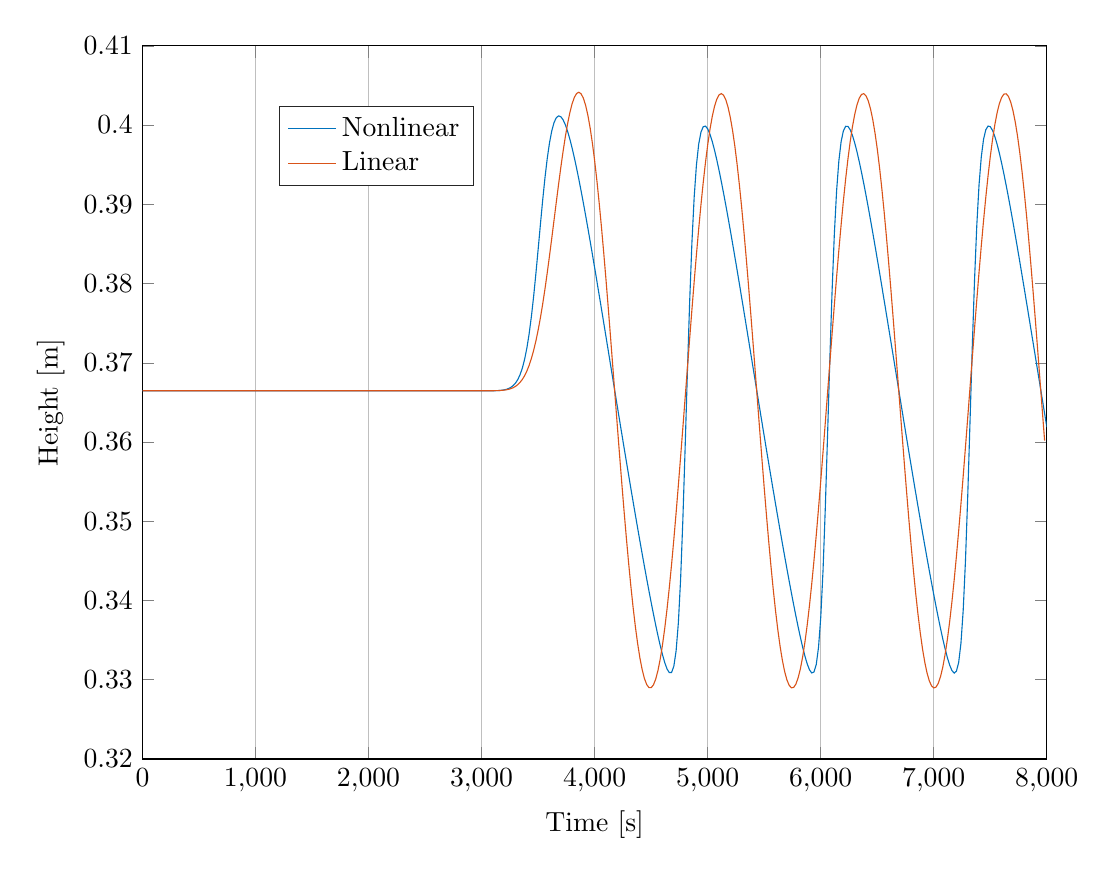
\begin{tikzpicture}

\begin{axis}[%
width=4.521in,
height=3.566in,
at={(0.758in,0.481in)},
scale only axis,
xmin=1,
xmajorgrids,
xmax=8000,
xlabel={Time [s]},
ymin=0.32,
ymax=0.41,
ylabel={Height [m]},
axis background/.style={fill=white},
legend style={at={(0.151,0.803)},anchor=south west,legend cell align=left,align=left,draw=white!15!black}
]
\addplot [color=mycolor1,solid]
  table[row sep=crcr]{%
1	0.366466627539343\\
21	0.366466665471691\\
41	0.366466692465574\\
61	0.366466711161801\\
81	0.366466723804557\\
101	0.366466732185832\\
121	0.36646673764237\\
141	0.366466741130459\\
161	0.366466743316878\\
181	0.366466744658372\\
201	0.366466745462716\\
221	0.366466745933408\\
241	0.366466746202002\\
261	0.366466746351381\\
281	0.366466746432328\\
301	0.366466746475058\\
321	0.366466746497021\\
341	0.366466746507986\\
361	0.366466746513251\\
381	0.366466746515595\\
401	0.366466746516464\\
421	0.366466746516784\\
441	0.366466746517842\\
461	0.366466746523015\\
481	0.366466746542095\\
501	0.366466746602594\\
521	0.366466746778925\\
541	0.366466747266689\\
561	0.366466748569185\\
581	0.366466751960835\\
601	0.366466760628919\\
621	0.366466782467414\\
641	0.366466824991748\\
661	0.366466877551302\\
681	0.366466909012503\\
701	0.366466897208555\\
721	0.366466852534906\\
741	0.366466804147601\\
761	0.366466772150041\\
781	0.366466758747709\\
801	0.366466757277496\\
821	0.366466761510951\\
841	0.366466768027839\\
861	0.366466774891905\\
881	0.366466780360355\\
901	0.366466782584759\\
921	0.366466779950668\\
941	0.366466771652426\\
961	0.366466758289697\\
981	0.366466742200663\\
1001	0.366466727015492\\
1021	0.366466716248985\\
1041	0.366466711712184\\
1061	0.36646671292079\\
1081	0.366466717849068\\
1101	0.366466724270585\\
1121	0.366466730692934\\
1141	0.366466736503687\\
1161	0.366466741612614\\
1181	0.366466746070639\\
1201	0.366466749918425\\
1221	0.366466753212207\\
1241	0.366466756057859\\
1261	0.366466758568098\\
1281	0.366466760782904\\
1301	0.366466762630246\\
1321	0.366466763956583\\
1341	0.366466764600551\\
1361	0.366466764466437\\
1381	0.366466763568626\\
1401	0.366466762037936\\
1421	0.366466760093622\\
1441	0.366466757992639\\
1461	0.366466755973411\\
1481	0.366466754212242\\
1501	0.366466752803997\\
1521	0.366466751767025\\
1541	0.366466751062805\\
1561	0.366466750618922\\
1581	0.366466750348598\\
1601	0.366466750165625\\
1621	0.366466749995936\\
1641	0.366466749786227\\
1661	0.3664667495087\\
1681	0.366466749160881\\
1701	0.366466748760672\\
1721	0.366466748338205\\
1741	0.366466747926767\\
1761	0.366466747555017\\
1781	0.366466747241989\\
1801	0.366466746995384\\
1821	0.366466746812749\\
1841	0.366466746684462\\
1861	0.366466746597258\\
1881	0.366466746537244\\
1901	0.366466746491858\\
1921	0.366466746450686\\
1941	0.366466746405459\\
1961	0.366466746349626\\
1981	0.366466746277887\\
2001	0.366466746185904\\
2021	0.366466746070288\\
2041	0.366466745928832\\
2061	0.366466745760932\\
2081	0.366466745568062\\
2101	0.366466745354198\\
2121	0.366466745126059\\
2141	0.366466744893064\\
2161	0.366466744666916\\
2181	0.366466744460798\\
2201	0.366466744288228\\
2221	0.366466744161677\\
2241	0.366466744091142\\
2261	0.366466744082878\\
2281	0.366466744138518\\
2301	0.366466744254728\\
2321	0.366466744423502\\
2341	0.36646674463305\\
2361	0.36646674486915\\
2381	0.366466745116762\\
2401	0.366466745361616\\
2421	0.366466745591559\\
2441	0.366466745797464\\
2461	0.366466745973624\\
2481	0.366466746117661\\
2501	0.366466746230052\\
2521	0.366466746313472\\
2541	0.366466746372187\\
2561	0.366466746411741\\
2581	0.366466746439263\\
2601	0.366466746464757\\
2621	0.366466746503873\\
2641	0.366466746582789\\
2661	0.366466746746095\\
2681	0.366466747069193\\
2701	0.36646674767828\\
2721	0.366466748783901\\
2741	0.366466750739029\\
2761	0.366466754138687\\
2781	0.366466759982299\\
2801	0.36646676991917\\
2821	0.366466786593398\\
2841	0.366466814088952\\
2861	0.36646685843496\\
2881	0.366466928083948\\
2901	0.366467034252727\\
2921	0.366467190986076\\
2941	0.366467414840061\\
2961	0.366467724280932\\
2981	0.366468138783252\\
3001	0.366468676751559\\
3021	0.366469356580593\\
3041	0.366470160960045\\
3061	0.366470781403547\\
3081	0.366471022304454\\
3101	0.366471811024978\\
3121	0.366476427538425\\
3141	0.366487208981108\\
3161	0.366506895988427\\
3181	0.366538154958313\\
3201	0.366586229651467\\
3221	0.366657715979119\\
3241	0.366763499523946\\
3261	0.366917391782519\\
3281	0.367139043129368\\
3301	0.367454993617361\\
3321	0.367897574460509\\
3341	0.36850855187551\\
3361	0.369337832554681\\
3381	0.37043866992242\\
3401	0.371865159415155\\
3421	0.373661877605495\\
3441	0.375850343116391\\
3461	0.378414236067563\\
3481	0.381291378533925\\
3501	0.384372804695217\\
3521	0.387512844594873\\
3541	0.3905512657543\\
3561	0.393339024106083\\
3581	0.395760573204265\\
3601	0.397742212920716\\
3621	0.399253919158054\\
3641	0.400302489298008\\
3661	0.400921093207355\\
3681	0.401154805407434\\
3701	0.401054639418849\\
3721	0.400670054854328\\
3741	0.400044850827336\\
3761	0.399219931578186\\
3781	0.398231007240009\\
3801	0.397106391211165\\
3821	0.395869603122493\\
3841	0.394540406299105\\
3861	0.393135051133942\\
3881	0.391665292279339\\
3901	0.390140640134986\\
3921	0.388569371321836\\
3941	0.386958604443187\\
3961	0.38531471749247\\
3981	0.383643494314967\\
4001	0.381950063243732\\
4021	0.380238783307623\\
4041	0.378513224443925\\
4061	0.376776293633958\\
4081	0.375030462811205\\
4101	0.373278012271646\\
4121	0.371521207603475\\
4141	0.369762211219868\\
4161	0.368003981050243\\
4181	0.366248027876198\\
4201	0.364495589895054\\
4221	0.36274817837337\\
4241	0.361007152561846\\
4261	0.359273873239861\\
4281	0.357549838340364\\
4301	0.355836692094989\\
4321	0.354136130444112\\
4341	0.352449809744458\\
4361	0.350779359466021\\
4381	0.349126509850378\\
4401	0.347493244675979\\
4421	0.345881887104931\\
4441	0.344295128405862\\
4461	0.342736107800051\\
4481	0.341208644935977\\
4501	0.339717633803796\\
4521	0.33826955870226\\
4541	0.336873179515492\\
4561	0.335540622633128\\
4581	0.334289313421881\\
4601	0.333145351925141\\
4621	0.332149220420964\\
4641	0.331364845137868\\
4661	0.330898154725945\\
4681	0.330920611138669\\
4701	0.331701861406759\\
4721	0.333627016627402\\
4741	0.337160391967049\\
4761	0.342687389504208\\
4781	0.350238925379372\\
4801	0.359278979022061\\
4821	0.368794883507088\\
4841	0.37768617476616\\
4861	0.385162896231032\\
4881	0.390901512494647\\
4901	0.394957571487544\\
4921	0.397587637909411\\
4941	0.399103627806496\\
4961	0.399788283600559\\
4981	0.399867543422794\\
5001	0.39950909035249\\
5021	0.398831004158808\\
5041	0.397918849649403\\
5061	0.396831762165564\\
5081	0.395610614486114\\
5101	0.394285153457823\\
5121	0.3928774871264\\
5141	0.391402867141369\\
5161	0.389872855411301\\
5181	0.388296811340508\\
5201	0.386682245098759\\
5221	0.385035455056554\\
5241	0.383361890492746\\
5261	0.381666299510196\\
5281	0.379952784260602\\
5301	0.378224870546435\\
5321	0.376485619899744\\
5341	0.374737747980308\\
5361	0.372983713654822\\
5381	0.371225798099233\\
5401	0.36946610982738\\
5421	0.367707346012034\\
5441	0.36595097244915\\
5461	0.364198476560114\\
5481	0.362451679502103\\
5501	0.360712151476488\\
5521	0.358981259374727\\
5541	0.357260283676455\\
5561	0.355550513137554\\
5581	0.353853314735917\\
5601	0.352170204157126\\
5621	0.350502906793907\\
5641	0.348853389344001\\
5661	0.347223875832671\\
5681	0.345616877505002\\
5701	0.344035250737081\\
5721	0.342482293026944\\
5741	0.340961912112083\\
5761	0.339478946792838\\
5781	0.338039744245102\\
5801	0.336653094188786\\
5821	0.335331662543733\\
5841	0.334094230460581\\
5861	0.332969329119605\\
5881	0.33200112977471\\
5901	0.331259545943237\\
5921	0.330859362295213\\
5941	0.330986746043631\\
5961	0.331929449934038\\
5981	0.334090502395966\\
6001	0.337936144363351\\
6021	0.343813694095991\\
6041	0.351668387281232\\
6061	0.360868048451852\\
6081	0.370353489513562\\
6101	0.37905274639098\\
6121	0.386250226872436\\
6141	0.391696415926776\\
6161	0.395492912117389\\
6181	0.39791438712643\\
6201	0.399272584189829\\
6221	0.399842045257527\\
6241	0.399838368584545\\
6261	0.399420391023125\\
6281	0.398698828491274\\
6301	0.397753915648429\\
6321	0.39664151960812\\
6341	0.395400219691452\\
6361	0.394058510709846\\
6381	0.392637268257605\\
6401	0.391151007525382\\
6421	0.389610922960775\\
6441	0.388026068082844\\
6461	0.386403786553424\\
6481	0.384750354678642\\
6501	0.383071309587512\\
6521	0.381371532327119\\
6541	0.37965522446482\\
6561	0.377925912612961\\
6581	0.37618653308801\\
6601	0.374439566745701\\
6621	0.372687159542499\\
6641	0.37093123369377\\
6661	0.369173762904317\\
6681	0.367417034013407\\
6701	0.365662198103127\\
6721	0.36391058042425\\
6741	0.362163892089778\\
6761	0.360423754996183\\
6781	0.358691793324237\\
6801	0.356969726303292\\
6821	0.355259390732162\\
6841	0.35356268781958\\
6861	0.351881499371196\\
6881	0.350217628278927\\
6901	0.348572810116784\\
6921	0.346948821893045\\
6941	0.345347668357579\\
6961	0.343771796843851\\
6981	0.342224323474826\\
7001	0.340709306127834\\
7021	0.339232116288827\\
7041	0.337799965520416\\
7061	0.336422693537365\\
7081	0.335114077562667\\
7101	0.333894157530986\\
7121	0.332793331053009\\
7141	0.331858832042384\\
7161	0.331166560746507\\
7181	0.330841014355229\\
7201	0.331083601276122\\
7221	0.332200931959585\\
7241	0.334612787291948\\
7261	0.33878182052881\\
7281	0.345008300801698\\
7301	0.353146585755168\\
7321	0.362473141745206\\
7341	0.371894864520334\\
7361	0.380379351083128\\
7381	0.387288734981073\\
7401	0.392443966115048\\
7421	0.395987436828022\\
7441	0.398207733177049\\
7461	0.399413773339763\\
7481	0.39987142748879\\
7501	0.399786479958598\\
7521	0.399309478906048\\
7541	0.398545717854504\\
7561	0.397571286774141\\
7581	0.396438242170758\\
7601	0.395181986798585\\
7621	0.393829305856599\\
7641	0.392398715789982\\
7661	0.390903890750215\\
7681	0.389355936704368\\
7701	0.387763859127099\\
7721	0.38613514005755\\
7741	0.384476100964206\\
7761	0.38279213085877\\
7781	0.381087856541197\\
7801	0.379367293514824\\
7821	0.37763396175543\\
7841	0.375890946504859\\
7861	0.374140924826797\\
7881	0.372386196920327\\
7901	0.370628746234173\\
7921	0.368870823401302\\
7941	0.367114475123368\\
7961	0.365360770569571\\
7981	0.363611061848541\\
8001	0.361866947544438\\
};
\addlegendentry{Nonlinear};

\addplot [color=mycolor2,solid]
  table[row sep=crcr]{%
1	0.366466627539343\\
21	0.366466627539343\\
41	0.366466627539343\\
61	0.366466627539343\\
81	0.366466627539343\\
101	0.366466627539343\\
121	0.366466627539343\\
141	0.366466627539343\\
161	0.366466627539343\\
181	0.366466627539343\\
201	0.366466627539343\\
221	0.366466627539343\\
241	0.366466627539343\\
261	0.366466627539343\\
281	0.366466627539343\\
301	0.366466627539343\\
321	0.366466627539343\\
341	0.366466627539343\\
361	0.366466627539343\\
381	0.366466627539343\\
401	0.366466627539343\\
421	0.366466627539343\\
441	0.366466627539343\\
461	0.366466627539343\\
481	0.366466627539343\\
501	0.366466627539343\\
521	0.366466627539343\\
541	0.366466627539343\\
561	0.366466627539343\\
581	0.366466627539343\\
601	0.366466627539343\\
621	0.366466627539343\\
641	0.366466627539343\\
661	0.366466627539343\\
681	0.366466627539343\\
701	0.366466627539343\\
721	0.366466627539343\\
741	0.366466627539343\\
761	0.366466627539343\\
781	0.366466627539343\\
801	0.366466627539343\\
821	0.366466627539343\\
841	0.366466627539343\\
861	0.366466627539343\\
881	0.366466627539343\\
901	0.366466627539343\\
921	0.366466627539343\\
941	0.366466627539343\\
961	0.366466627539343\\
981	0.366466627539343\\
1001	0.366466627539343\\
1021	0.366466627539343\\
1041	0.366466627539343\\
1061	0.366466627539343\\
1081	0.366466627539343\\
1101	0.366466627539343\\
1121	0.366466627539343\\
1141	0.366466627539343\\
1161	0.366466627539343\\
1181	0.366466627539343\\
1201	0.366466627539343\\
1221	0.366466627539343\\
1241	0.366466627539343\\
1261	0.366466627539343\\
1281	0.366466627539343\\
1301	0.366466627539343\\
1321	0.366466627539343\\
1341	0.366466627539343\\
1361	0.366466627539343\\
1381	0.366466627539343\\
1401	0.366466627539343\\
1421	0.366466627539343\\
1441	0.366466627539343\\
1461	0.366466627539343\\
1481	0.366466627539343\\
1501	0.366466627539343\\
1521	0.366466627539343\\
1541	0.366466627539343\\
1561	0.366466627539343\\
1581	0.366466627539343\\
1601	0.366466627539343\\
1621	0.366466627539343\\
1641	0.366466627539343\\
1661	0.366466627539343\\
1681	0.366466627539343\\
1701	0.366466627539343\\
1721	0.366466627539343\\
1741	0.366466627539343\\
1761	0.366466627539343\\
1781	0.366466627539343\\
1801	0.366466627539343\\
1821	0.366466627539343\\
1841	0.366466627539343\\
1861	0.366466627539343\\
1881	0.366466627539343\\
1901	0.366466627539343\\
1921	0.366466627539343\\
1941	0.366466627539343\\
1961	0.366466627539343\\
1981	0.366466627539343\\
2001	0.366466627539343\\
2021	0.366466627539343\\
2041	0.366466627539343\\
2061	0.366466627539343\\
2081	0.366466627539343\\
2101	0.366466627539343\\
2121	0.366466627539343\\
2141	0.366466627539343\\
2161	0.366466627539343\\
2181	0.366466627539343\\
2201	0.366466627539343\\
2221	0.366466627539343\\
2241	0.366466627539343\\
2261	0.366466627539343\\
2281	0.366466627539343\\
2301	0.366466627539343\\
2321	0.366466627539343\\
2341	0.366466627539343\\
2361	0.366466627539343\\
2381	0.366466627539343\\
2401	0.366466627539343\\
2421	0.366466627539343\\
2441	0.366466627539343\\
2461	0.366466627539343\\
2481	0.366466627539343\\
2501	0.366466627539344\\
2521	0.366466627539346\\
2541	0.366466627539352\\
2561	0.366466627539367\\
2581	0.366466627539406\\
2601	0.366466627539506\\
2621	0.366466627539753\\
2641	0.366466627540356\\
2661	0.366466627541801\\
2681	0.366466627545203\\
2701	0.36646662755307\\
2721	0.366466627570933\\
2741	0.366466627610775\\
2761	0.36646662769805\\
2781	0.366466627885832\\
2801	0.366466628282679\\
2821	0.366466629106458\\
2841	0.366466630786123\\
2861	0.366466634150207\\
2881	0.366466640768553\\
2901	0.366466653558754\\
2921	0.366466677839224\\
2941	0.366466723118069\\
2961	0.366466806064708\\
2981	0.36646695533534\\
3001	0.366467219229196\\
3021	0.366467677551623\\
3041	0.366468459553763\\
3061	0.366469770390096\\
3081	0.366471929138866\\
3101	0.366475421982078\\
3121	0.366480974508741\\
3141	0.366489647104487\\
3161	0.366502956796009\\
3181	0.366523027482528\\
3201	0.36655276798044\\
3221	0.366596073581188\\
3241	0.366658041875905\\
3261	0.366745187657059\\
3281	0.366865635273379\\
3301	0.36702926070058\\
3321	0.367247750875542\\
3341	0.367534545762865\\
3361	0.367904630390547\\
3381	0.368374150646985\\
3401	0.368959838382449\\
3421	0.369678247951269\\
3441	0.370544826519821\\
3461	0.371572862132087\\
3481	0.372772373883958\\
3501	0.374149024538009\\
3521	0.375703144660012\\
3541	0.377428956784265\\
3561	0.379314077344984\\
3581	0.38133935376884\\
3601	0.38347906633576\\
3621	0.385701492533075\\
3641	0.387969799702821\\
3661	0.390243203893882\\
3681	0.392478312407949\\
3701	0.394630556796896\\
3721	0.396655622738953\\
3741	0.398510792465058\\
3761	0.400156132117748\\
3781	0.401555477678416\\
3801	0.402677195711344\\
3821	0.403494716236732\\
3841	0.403986852338963\\
3861	0.404137933333533\\
3881	0.403937785095086\\
3901	0.403381592938361\\
3921	0.402469680258693\\
3941	0.401207231276515\\
3961	0.399603980007785\\
3981	0.397673881135668\\
4001	0.395434772626878\\
4021	0.392908035224715\\
4041	0.390118250560682\\
4061	0.387092857521657\\
4081	0.383861805500206\\
4101	0.380457202977927\\
4121	0.376912960270778\\
4141	0.373264425957107\\
4161	0.36954801732205\\
4181	0.365800845952344\\
4201	0.362060340322025\\
4221	0.358363867782038\\
4241	0.354748358794466\\
4261	0.351249936541774\\
4281	0.347903555208967\\
4301	0.344742650300615\\
4321	0.341798804333533\\
4341	0.339101431155141\\
4361	0.336677481990077\\
4381	0.334551176123472\\
4401	0.332743758896428\\
4421	0.331273289423679\\
4441	0.330154460150449\\
4461	0.329398450049507\\
4481	0.329012812924289\\
4501	0.329001401933752\\
4521	0.329364331092909\\
4541	0.330097974133665\\
4561	0.331195000737319\\
4581	0.332644449776703\\
4601	0.334431838836153\\
4621	0.336539308915026\\
4641	0.338945802868934\\
4661	0.341627275805773\\
4681	0.344556935334334\\
4701	0.347705509265027\\
4721	0.351041538087915\\
4741	0.354531689305745\\
4761	0.358141090481239\\
4781	0.361833677670961\\
4801	0.365572555764319\\
4821	0.369320367127311\\
4841	0.373039664867661\\
4861	0.376693286991785\\
4881	0.380244727715143\\
4901	0.383658502215979\\
4921	0.386900501187925\\
4941	0.389938331648914\\
4961	0.392741640601155\\
4981	0.395282418308246\\
5001	0.397535278159209\\
5021	0.399477710323108\\
5041	0.401090306659845\\
5061	0.402356954639877\\
5081	0.403264998335285\\
5101	0.403805364873624\\
5121	0.403972655091064\\
5141	0.403765197479053\\
5161	0.403185064885471\\
5181	0.402238053803429\\
5201	0.400933626454617\\
5221	0.399284816245919\\
5241	0.397308097543916\\
5261	0.395023221068461\\
5281	0.392453016550019\\
5301	0.38962316462254\\
5321	0.386561940231059\\
5341	0.38329993011779\\
5361	0.379869727209507\\
5381	0.376305604959795\\
5401	0.372643174900031\\
5421	0.368919030820735\\
5441	0.365170383138508\\
5461	0.361434687101853\\
5481	0.35774926855071\\
5501	0.354150950969006\\
5521	0.350675687556572\\
5541	0.347358201996655\\
5561	0.344231641508354\\
5581	0.341327245650566\\
5601	0.338674034186636\\
5621	0.336298517128476\\
5641	0.33422442985729\\
5661	0.33247249596749\\
5681	0.331060220203389\\
5701	0.330001713557588\\
5721	0.329307552278593\\
5741	0.328984672196448\\
5761	0.329036299422201\\
5781	0.329461918113679\\
5801	0.330257275629608\\
5821	0.331414425020598\\
5841	0.332921804432438\\
5861	0.334764352628319\\
5881	0.336923659475731\\
5901	0.339378149894427\\
5921	0.342103299427492\\
5941	0.345071879281605\\
5961	0.348254228388145\\
5981	0.351618549766786\\
6001	0.355131228230408\\
6021	0.35875716625694\\
6041	0.362460134672197\\
6061	0.366203134639811\\
6081	0.369948767341379\\
6101	0.373659607653087\\
6121	0.377298578085182\\
6141	0.380829319247989\\
6161	0.384216553142919\\
6181	0.387426435648562\\
6201	0.39042689467997\\
6221	0.39318795064232\\
6241	0.39568201597712\\
6261	0.397884170807974\\
6281	0.399772411931746\\
6301	0.401327872667297\\
6321	0.402535011365126\\
6341	0.40338176669439\\
6361	0.40385967815574\\
6381	0.40396397061583\\
6401	0.403693602018873\\
6421	0.403051273798518\\
6441	0.402043403886018\\
6461	0.40068006258438\\
6481	0.398974871949231\\
6501	0.396944869681735\\
6521	0.394610338893519\\
6541	0.391994605444527\\
6561	0.389123804878734\\
6581	0.386026621286432\\
6601	0.382734000702284\\
6621	0.37927884190277\\
6641	0.375695667692492\\
6661	0.372020279963719\\
6681	0.368289401975715\\
6701	0.364540311428072\\
6721	0.360810467994257\\
6741	0.357137139036939\\
6761	0.353557027244818\\
6781	0.350105903911493\\
6801	0.346818251520522\\
6821	0.343726919207841\\
6841	0.34086279454406\\
6861	0.338254494916066\\
6881	0.335928081591553\\
6901	0.333906799323449\\
6921	0.33221084409603\\
6941	0.33085716133332\\
6961	0.329859276586016\\
6981	0.329227160388656\\
7001	0.328967128637335\\
7021	0.329081779483356\\
7041	0.329569967373365\\
7061	0.330426814495338\\
7081	0.331643759516069\\
7101	0.333208643123178\\
7121	0.335105829516945\\
7141	0.337316362638051\\
7161	0.339818155570254\\
7181	0.342586211225559\\
7201	0.345592872106854\\
7221	0.348808096652485\\
7241	0.352199759401603\\
7261	0.355733971981154\\
7281	0.359375421707298\\
7301	0.363087724418075\\
7321	0.366833788011923\\
7341	0.370576183059695\\
7361	0.374277516787147\\
7381	0.377900806691172\\
7401	0.381409850056748\\
7421	0.384769585682503\\
7441	0.387946444200646\\
7461	0.390908683490992\\
7481	0.393626705837738\\
7501	0.396073353660056\\
7521	0.398224180861657\\
7541	0.400057697088114\\
7561	0.40155558245137\\
7581	0.402702870576012\\
7601	0.403488098138341\\
7621	0.403903419404116\\
7641	0.403944684620536\\
7661	0.403611481479199\\
7681	0.402907139235752\\
7701	0.401838695445065\\
7721	0.400416825644316\\
7741	0.398655736686546\\
7761	0.396573024790481\\
7781	0.394189499724935\\
7801	0.391528976884473\\
7821	0.388618039333867\\
7841	0.385485772198892\\
7861	0.382163472057373\\
7881	0.378684334234116\\
7901	0.375083121124203\\
7921	0.371395814858623\\
7941	0.367659257782722\\
7961	0.36391078433966\\
7981	0.360187848037\\
};
\addlegendentry{Linear};

\end{axis}
\end{tikzpicture}%
% \caption{Output height for the linear and Preissmann scheme simulation.}
% \label{fig:height_output_nonlinear_and_linear_model}
% \end{figure}
 


 %The fluctuations of the response of the nonlinear and linear are not identical as the top and bottom of the curves peaks at different times. However, the linear output looks very similar in phase as the input signal shown in figure \ref{fig:height_input_for_comparision} where the nonlinear has a faster response up going, and a slower one down going. It should be noted, that each time the response for both the models crosses the linearization point, they cross the same point. Hence it can be verified that the two models follows a similar pattern. It can be concluded that the plot of the nonlinear and linear responses are very similar, and therefore the linear model will be used to construct the MPC controller.  
In figure \ref{fig:linear_nonlinear_comparison_input_to_first_pipe} the input to the first pipe is seen. 

\begin{figure}[H]
 \centering
 % This file was created by matlab2tikz.
%
%The latest updates can be retrieved from
%  http://www.mathworks.com/matlabcentral/fileexchange/22022-matlab2tikz-matlab2tikz
%where you can also make suggestions and rate matlab2tikz.
%
\definecolor{mycolor1}{rgb}{0.00000,0.44700,0.74100}%
%
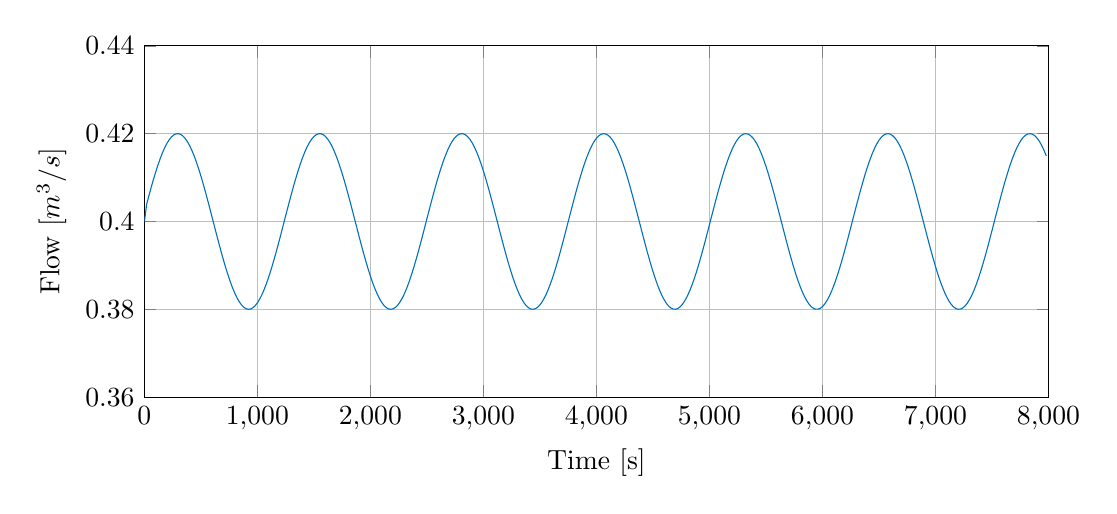
\begin{tikzpicture}

\begin{axis}[%
width=4.521in,
height=1.7566in,
at={(0.758in,0.481in)},
scale only axis,
xmin=0,
xmajorgrids,
ymajorgrids,
xmax=8000,
ymin=0.36,
ymax=0.44,
xlabel={Time [s]},
ylabel={Flow $[m^3/s]$},
axis background/.style={fill=white}
]
\addplot [color=mycolor1,solid,forget plot]
  table[row sep=crcr]{%
1	0.4\\
21	0.403973386615901\\
41	0.405910404133227\\
61	0.407788366846173\\
81	0.409588510772084\\
101	0.411292849467901\\
121	0.412884353744754\\
141	0.41434712181799\\
161	0.41566653819255\\
181	0.416829419696158\\
201	0.417824147201229\\
221	0.418640781719345\\
241	0.419271163708344\\
261	0.419708994599769\\
281	0.419949899732081\\
301	0.41999147206083\\
321	0.419833296209049\\
341	0.419476952617564\\
361	0.418926001753748\\
381	0.418185948536514\\
401	0.417264187332977\\
421	0.416169928076392\\
441	0.414914104243534\\
461	0.413509263611023\\
481	0.411969442882079\\
501	0.410310027436429\\
521	0.408547597604677\\
541	0.406699763003118\\
561	0.40478498658428\\
581	0.402822400161197\\
601	0.400831613248666\\
621	0.398832517131448\\
641	0.396845086117135\\
661	0.394889177959463\\
681	0.392984335446208\\
701	0.391149591134103\\
721	0.38940327718183\\
741	0.387762842181146\\
761	0.386244676816321\\
781	0.384863950093841\\
801	0.383634457778712\\
821	0.382568484551728\\
841	0.381676681265011\\
861	0.38096795852221\\
881	0.380449397646698\\
901	0.380126179927331\\
921	0.380001534848718\\
941	0.380076707823283\\
961	0.380350947747513\\
981	0.380821514506737\\
1001	0.381483706353445\\
1021	0.382330906885597\\
1041	0.383354651155522\\
1061	0.38454471024888\\
1081	0.385889193488592\\
1101	0.387374667242554\\
1121	0.388986289148047\\
1141	0.390707956411725\\
1161	0.392522466703395\\
1181	0.394411690036022\\
1201	0.396356749914558\\
1221	0.39833821194365\\
1241	0.400336278009687\\
1261	0.40233098409701\\
1281	0.404302399761756\\
1301	0.406230827270268\\
1321	0.408096998412332\\
1341	0.409882267022772\\
1361	0.411568795287764\\
1381	0.413139731974376\\
1401	0.414579380802518\\
1421	0.415873357276983\\
1441	0.417008732412571\\
1461	0.417974161916233\\
1481	0.418759999535495\\
1501	0.41935839344063\\
1521	0.41976336467754\\
1541	0.419970866907492\\
1561	0.419978826836795\\
1581	0.419787164932468\\
1601	0.419397796216902\\
1621	0.418814611133595\\
1641	0.418043436675126\\
1661	0.417091978161766\\
1681	0.41596974225247\\
1701	0.414687941957482\\
1721	0.413259384601644\\
1741	0.411698343857835\\
1761	0.410020417129158\\
1781	0.408242369704835\\
1801	0.406381967246987\\
1821	0.404457798282005\\
1841	0.402489088470141\\
1861	0.400495508509067\\
1881	0.398496977590764\\
1901	0.39651346437554\\
1921	0.394564787471781\\
1941	0.392670417414961\\
1961	0.390849282124494\\
1981	0.389119577782213\\
2001	0.387498587022142\\
2021	0.386002506248129\\
2041	0.384646283804728\\
2061	0.383443470618287\\
2081	0.382406084800567\\
2101	0.381544491567744\\
2121	0.380867299674596\\
2141	0.38038127539867\\
2161	0.380091274933872\\
2181	0.380000195868986\\
2201	0.38010894823592\\
2221	0.380416445416974\\
2241	0.380919615001958\\
2261	0.381613429486707\\
2281	0.382490956506231\\
2301	0.383543428100626\\
2321	0.384760328321619\\
2341	0.386129498304458\\
2361	0.387637257755259\\
2381	0.389268541639991\\
2401	0.391007050709308\\
2421	0.392835414355263\\
2441	0.394735364172684\\
2461	0.396687916491034\\
2481	0.398673562052976\\
2501	0.400672460944423\\
2521	0.402664640828399\\
2541	0.404630196502031\\
2561	0.406549488782754\\
2581	0.408403340736533\\
2601	0.410173229287447\\
2621	0.411841470294144\\
2641	0.413391395243932\\
2661	0.414807517799049\\
2681	0.416075688531032\\
2701	0.41718323629713\\
2721	0.418119094846169\\
2741	0.418873913388882\\
2761	0.4194401500279\\
2781	0.419812147113897\\
2801	0.419986187774958\\
2821	0.419960533054327\\
2841	0.419735439285492\\
2861	0.419313155530986\\
2881	0.418697901110494\\
2901	0.41789582344281\\
2921	0.416914936622859\\
2941	0.415765041347506\\
2961	0.41445762699024\\
2981	0.413005756803142\\
3001	0.4114239373932\\
3021	0.409727973777076\\
3041	0.407934811462612\\
3061	0.406062367134914\\
3081	0.404129349638756\\
3101	0.402155073045989\\
3121	0.400159263675719\\
3141	0.398161862995446\\
3161	0.396182828372516\\
3181	0.394241933666699\\
3201	0.39235857165632\\
3221	0.390551560272031\\
3241	0.388838954574264\\
3261	0.387237866353041\\
3281	0.385764293152618\\
3301	0.384432958429314\\
3321	0.383257164439605\\
3341	0.38224865932837\\
3361	0.381417519745313\\
3381	0.380772050162409\\
3401	0.380318699898367\\
3421	0.380061998679168\\
3441	0.38000451137854\\
3461	0.380146812390587\\
3481	0.380487479890637\\
3501	0.381023110041638\\
3521	0.381748351004176\\
3541	0.382655956410288\\
3561	0.38373685776677\\
3581	0.384980255064567\\
3601	0.38637372468889\\
3621	0.387903343551874\\
3641	0.389553828207465\\
3661	0.391308687558562\\
3681	0.393150387630608\\
3701	0.395060526765268\\
3721	0.397020019483716\\
3741	0.399009287182433\\
3761	0.401008453756136\\
3781	0.402997544193259\\
3801	0.404956684159659\\
3821	0.406866298576398\\
3841	0.408707307207458\\
3861	0.410461315303154\\
3881	0.412110797394392\\
3901	0.413639272401363\\
3921	0.415031468307043\\
3941	0.416273474750142\\
3961	0.417352882012833\\
3981	0.418258905014553\\
4001	0.418982491072958\\
4021	0.41951641035534\\
4041	0.419855328116718\\
4061	0.419995858002853\\
4081	0.419936595885576\\
4101	0.419678133892372\\
4121	0.419223054490042\\
4141	0.418575904681545\\
4161	0.417743150573847\\
4181	0.416733112770721\\
4201	0.415555883236022\\
4221	0.41422322445812\\
4241	0.412748451923005\\
4261	0.411146301070353\\
4281	0.409432780061884\\
4301	0.407625009833099\\
4321	0.405741053026555\\
4341	0.403799733515909\\
4361	0.401820448323997\\
4381	0.399822973814192\\
4401	0.397827268091518\\
4421	0.395853271587865\\
4441	0.393920707823779\\
4461	0.392048886337571\\
4481	0.39025650975079\\
4501	0.388561486897809\\
4521	0.386980753886675\\
4541	0.385530104879115\\
4561	0.384224034280492\\
4581	0.383075591916497\\
4601	0.382096252643606\\
4621	0.381295801696109\\
4641	0.380682236915279\\
4661	0.380261688837587\\
4681	0.380038359440412\\
4701	0.380014480157267\\
4721	0.380190289582057\\
4741	0.380564031085123\\
4761	0.381131970364909\\
4781	0.381888432759868\\
4801	0.382825859947801\\
4821	0.383934885466121\\
4841	0.385204428298442\\
4861	0.38662180359244\\
4881	0.388172849402698\\
4901	0.389842068192188\\
4921	0.391612781678535\\
4941	0.393467297477906\\
4961	0.395387085881452\\
4981	0.397352964998045\\
5001	0.399345292413383\\
5021	0.40134416145051\\
5041	0.403329600070743\\
5061	0.405281770427689\\
5081	0.407181167080443\\
5101	0.409008811885508\\
5121	0.410746443620129\\
5141	0.412376700442401\\
5161	0.413883293365045\\
5181	0.415251169009592\\
5201	0.416466660014762\\
5221	0.417517621596218\\
5241	0.41839355289324\\
5261	0.419085701889854\\
5281	0.419587152862078\\
5301	0.419892895477557\\
5321	0.41999987485714\\
5341	0.419907022098231\\
5361	0.419615264954903\\
5381	0.41912751856809\\
5401	0.418448656338462\\
5421	0.417585461233014\\
5441	0.416546558011908\\
5461	0.415342327052711\\
5481	0.413984800633102\\
5501	0.412487542708328\\
5521	0.410865513384645\\
5541	0.409134919442884\\
5561	0.407313052405652\\
5581	0.405418115766157\\
5601	0.403469043104918\\
5621	0.401485308911687\\
5641	0.399486734002789\\
5661	0.397493287478071\\
5681	0.395524887196264\\
5701	0.393601200762316\\
5721	0.391741449015189\\
5741	0.389964213979589\\
5761	0.388287253200514\\
5781	0.386727322315741\\
5801	0.385300007639024\\
5821	0.384019570426808\\
5841	0.382898804384459\\
5861	0.381948907835796\\
5881	0.381179371833141\\
5901	0.380597885325856\\
5921	0.380210258334909\\
5941	0.380020363901061\\
5961	0.380030099386724\\
5981	0.380239367518143\\
6001	0.380646077357324\\
6021	0.381246165193994\\
6041	0.382033635148853\\
6061	0.383000619082413\\
6081	0.384137455210854\\
6101	0.385432784643368\\
6121	0.386873664876444\\
6141	0.388445699111085\\
6161	0.390133180100864\\
6181	0.391919247093539\\
6201	0.393786054298113\\
6221	0.395714949194082\\
6241	0.397686658901255\\
6261	0.399681482747998\\
6281	0.401679489113835\\
6301	0.403660714579612\\
6321	0.40560536339538\\
6341	0.407494005272989\\
6361	0.409307769527099\\
6381	0.411028533624834\\
6401	0.412639104260138\\
6421	0.414123389143607\\
6441	0.415466557791324\\
6461	0.416655189706156\\
6481	0.417677408470917\\
6501	0.418523000413611\\
6521	0.419183516659062\\
6541	0.419652357547283\\
6561	0.419924838575097\\
6581	0.419998237202145\\
6601	0.419871820053608\\
6621	0.419546850247845\\
6641	0.419026574775736\\
6661	0.418316192057816\\
6681	0.417422800003384\\
6701	0.416355325090529\\
6721	0.415124433175721\\
6741	0.413742422924095\\
6761	0.412223102925252\\
6781	0.410581653722401\\
6801	0.408834476133384\\
6821	0.406999027379133\\
6841	0.405093646656881\\
6861	0.403137371900968\\
6881	0.401149749562099\\
6901	0.399150639305661\\
6921	0.39716001558052\\
6941	0.395197768040925\\
6961	0.393283502815657\\
6981	0.391436346610077\\
7001	0.389674755598401\\
7021	0.388016331015715\\
7041	0.386477643292245\\
7061	0.385074066487102\\
7081	0.383819624675762\\
7101	0.382726851826141\\
7121	0.381806666563329\\
7141	0.381068263074301\\
7161	0.380519019242633\\
7181	0.380164422931138\\
7201	0.380008017148944\\
7221	0.380051364650927\\
7241	0.380294032323176\\
7261	0.380733595510525\\
7281	0.381365662242906\\
7301	0.382183917118463\\
7321	0.383180184404958\\
7341	0.384344509728987\\
7361	0.385665259536787\\
7381	0.38712923733286\\
7401	0.388721815534995\\
7421	0.390427081628232\\
7441	0.392227997157453\\
7461	0.394106567969995\\
7481	0.396044024007271\\
7501	0.398021006848994\\
7521	0.400017763136114\\
7541	0.40201434193985\\
7561	0.403990794104776\\
7581	0.405927371574188\\
7601	0.407804724706159\\
7621	0.409604095608765\\
7641	0.41130750556274\\
7661	0.412897934658897\\
7681	0.414359491855433\\
7701	0.415677573755966\\
7721	0.416839010521846\\
7741	0.417832197460829\\
7761	0.418647210977324\\
7781	0.419275907725682\\
7801	0.419712005975813\\
7821	0.419951148378156\\
7841	0.419990945500878\\
7861	0.419830999704283\\
7881	0.4194729091139\\
7901	0.418920251652538\\
7921	0.418178549290868\\
7941	0.417255212873714\\
7961	0.41615946807334\\
7981	0.414902263209587\\
};
\end{axis}
\end{tikzpicture}%
\caption{Input flow to the first pipe.}
\label{fig:linear_nonlinear_comparison_input_to_first_pipe}
\end{figure}
A sinusoidal input flow to the simulation setup is given, to compare the response of the nonlinear and linear model. 
In the following figures, comparisons are made between the nonlinear and linear model at different places in the simulation setup. In figure \ref{fig:linear_nonlinear_comparison_input_first_pipe_into_tank} the output of the first pipe is shown.

\begin{figure}[H]
 \centering
 % This file was created by matlab2tikz.
%
%The latest updates can be retrieved from
%  http://www.mathworks.com/matlabcentral/fileexchange/22022-matlab2tikz-matlab2tikz
%where you can also make suggestions and rate matlab2tikz.
%
\definecolor{mycolor1}{rgb}{0.00000,0.44700,0.74100}%
\definecolor{mycolor2}{rgb}{0.85000,0.32500,0.09800}%
%
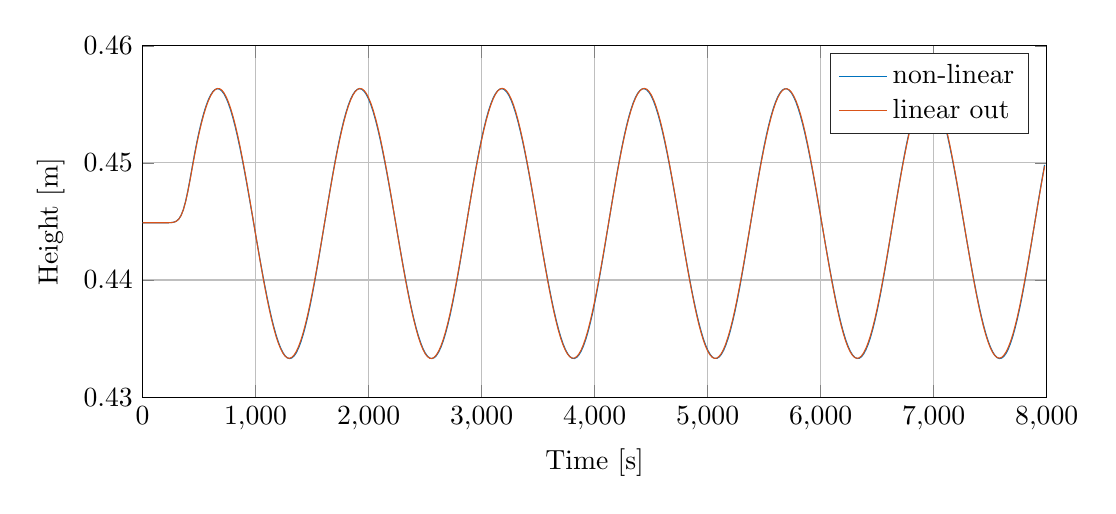
\begin{tikzpicture}

\begin{axis}[%
width=4.521in,
height=1.7566in,
at={(0.758in,0.481in)},
scale only axis,
xmin=0,
xmax=8000,
xlabel={Time [s]},
xmajorgrids,
ymin=0.43,
ymax=0.46,
ylabel={Height [m]},
ymajorgrids,
axis background/.style={fill=white},
legend style={legend cell align=left,align=left,draw=white!15!black}
]
\addplot [color=mycolor1,solid]
  table[row sep=crcr]{%
1	0.444890389772348\\
21	0.444890513105407\\
41	0.444890506028277\\
61	0.444890483539142\\
81	0.444890480180384\\
101	0.444890484549755\\
121	0.444890486153938\\
141	0.444890488187149\\
161	0.444890504664314\\
181	0.444890592226957\\
201	0.444890982364645\\
221	0.444892484368095\\
241	0.444897513208079\\
261	0.444912247332715\\
281	0.44495021707324\\
301	0.445036612933934\\
321	0.445210720248507\\
341	0.445522251378143\\
361	0.446018349496678\\
381	0.446723435380787\\
401	0.447621701901021\\
421	0.448655079484728\\
441	0.449741835128255\\
461	0.450806031355439\\
481	0.451799144263548\\
501	0.452702070386736\\
521	0.453512121631284\\
541	0.454229026870217\\
561	0.454849176245437\\
581	0.455366945609026\\
601	0.455777383168636\\
621	0.456077162609621\\
641	0.4562642983716\\
661	0.456337822034991\\
681	0.456297711358788\\
701	0.456144901035072\\
721	0.455881324013118\\
741	0.45550999835959\\
761	0.455035099955435\\
781	0.454461930626688\\
801	0.453796747739217\\
821	0.453046502054425\\
841	0.45221860533919\\
861	0.451320860272442\\
881	0.450361580453185\\
901	0.449349765856936\\
921	0.448295129482088\\
941	0.447207881921158\\
961	0.446098387500628\\
981	0.444976920226752\\
1001	0.443853654546849\\
1021	0.442738804741204\\
1041	0.441642695684339\\
1061	0.440575643739362\\
1081	0.439547742855924\\
1101	0.438568744696583\\
1121	0.437648092235126\\
1141	0.43679497083553\\
1161	0.43601820621578\\
1181	0.43532600044429\\
1201	0.434725669743442\\
1221	0.4342235459283\\
1241	0.4338250443032\\
1261	0.433534762217795\\
1281	0.433356475973452\\
1301	0.43329301863983\\
1321	0.433346112128187\\
1341	0.433516233625523\\
1361	0.433802546534754\\
1381	0.434202884036726\\
1401	0.434713766141664\\
1421	0.435330440621841\\
1441	0.436046931824876\\
1461	0.436856080427625\\
1481	0.437749576972346\\
1501	0.438718024815561\\
1521	0.439751064744405\\
1541	0.440837550909304\\
1561	0.441965747435319\\
1581	0.44312353243093\\
1601	0.44429858610053\\
1621	0.445478495604206\\
1641	0.446650744483934\\
1661	0.447802704273979\\
1681	0.448921824831973\\
1701	0.449996055560665\\
1721	0.4510142665232\\
1741	0.451966400742813\\
1761	0.452843343360739\\
1781	0.453636741725098\\
1801	0.454338982376328\\
1821	0.454943320892678\\
1841	0.455444049229152\\
1861	0.45583664108534\\
1881	0.456117868954708\\
1901	0.45628584381726\\
1921	0.456339907639262\\
1941	0.456280416738802\\
1961	0.456108584295105\\
1981	0.455826519958659\\
2001	0.455437413203808\\
2021	0.454945645843403\\
2041	0.454356677044245\\
2061	0.453676774614264\\
2081	0.452912808260128\\
2101	0.45207222519866\\
2121	0.451163123107327\\
2141	0.450194260118633\\
2161	0.449174942483414\\
2181	0.44811484418761\\
2201	0.447023832622007\\
2221	0.445911859124028\\
2241	0.444788967984734\\
2261	0.443665413175901\\
2281	0.442551742791173\\
2301	0.441458683628702\\
2321	0.440396837076628\\
2341	0.439376400121379\\
2361	0.438407091047066\\
2381	0.437498222247314\\
2401	0.436658717323784\\
2421	0.435896975935086\\
2441	0.435220688656884\\
2461	0.434636758074629\\
2481	0.434151357704681\\
2501	0.433770013415332\\
2521	0.433497563745665\\
2541	0.433337954641688\\
2561	0.433293961205547\\
2581	0.433366992134949\\
2601	0.43355707061449\\
2621	0.433862936396884\\
2641	0.434282124787469\\
2661	0.434810945465905\\
2681	0.435444431662193\\
2701	0.43617637582906\\
2721	0.436999463577042\\
2741	0.437905401908063\\
2761	0.438884947780973\\
2781	0.439927855583771\\
2801	0.441022867959747\\
2821	0.442157888136448\\
2841	0.44332035413576\\
2861	0.444497644483452\\
2881	0.445677272673719\\
2901	0.446846817264341\\
2921	0.447993827883114\\
2941	0.449105989715532\\
2961	0.450171525047388\\
2981	0.451179518034144\\
3001	0.452119946390693\\
3021	0.452983565354992\\
3041	0.453761932016254\\
3061	0.454447607111244\\
3081	0.455034300734856\\
3101	0.455516816322962\\
3121	0.45589094136335\\
3141	0.456153501256189\\
3161	0.456302549998853\\
3181	0.456337470078301\\
3201	0.456258860204721\\
3221	0.456068325305178\\
3241	0.455768346667694\\
3261	0.455362278565751\\
3281	0.45485440754496\\
3301	0.454250007361666\\
3321	0.45355534317873\\
3341	0.452777577140993\\
3361	0.451924577136784\\
3381	0.451004716011715\\
3401	0.450026756406294\\
3421	0.448999829815477\\
3441	0.447933449197968\\
3461	0.446837505655131\\
3481	0.445722231080723\\
3501	0.444598110993818\\
3521	0.443475741110116\\
3541	0.442365662189676\\
3561	0.441278232670896\\
3581	0.440223567945634\\
3601	0.439211523488113\\
3621	0.4382516809443\\
3641	0.437353313421694\\
3661	0.436525324038582\\
3681	0.435776156910669\\
3701	0.435113684321954\\
3721	0.434545081150217\\
3741	0.434076700594065\\
3761	0.433713967049432\\
3781	0.433461299771415\\
3801	0.43332205932846\\
3821	0.433298483970778\\
3841	0.43339160537411\\
3861	0.433601203275144\\
3881	0.433925866878906\\
3901	0.434363112610843\\
3921	0.434909390152479\\
3941	0.435559887168259\\
3961	0.436308287029692\\
3981	0.437146763726363\\
4001	0.438066310690831\\
4021	0.439057172270449\\
4041	0.440109051996531\\
4061	0.441211023601883\\
4081	0.442351376476064\\
4101	0.443517656900371\\
4121	0.44469694396713\\
4141	0.44587621067233\\
4161	0.447042630409426\\
4181	0.448183798971271\\
4201	0.449287894733353\\
4221	0.450343772209478\\
4241	0.451340962422148\\
4261	0.452269602625495\\
4281	0.453120402536078\\
4301	0.453884762882528\\
4321	0.454555039967992\\
4341	0.455124808414372\\
4361	0.455588979396579\\
4381	0.45594377182804\\
4401	0.456186628545273\\
4421	0.456316130034204\\
4441	0.456331897545565\\
4461	0.456234504455661\\
4481	0.456025457191654\\
4501	0.455707261141933\\
4521	0.455283495683509\\
4541	0.454758805495101\\
4561	0.454138793130599\\
4581	0.453429877793618\\
4601	0.452639186379266\\
4621	0.451774488769081\\
4641	0.450844147136555\\
4661	0.449857052611935\\
4681	0.448822548890726\\
4701	0.447750354531074\\
4721	0.446650489496358\\
4741	0.445533204159083\\
4761	0.444408906206146\\
4781	0.443288079076946\\
4801	0.442181189540063\\
4821	0.441098592173128\\
4841	0.440050440118039\\
4861	0.439046604513022\\
4881	0.43809661193001\\
4901	0.437209620889085\\
4921	0.436394426400625\\
4941	0.435659415136744\\
4961	0.435012398196607\\
4981	0.434460373603032\\
5001	0.434009382256267\\
5021	0.433664546306504\\
5041	0.433430166698647\\
5061	0.433309665549796\\
5081	0.433305328813018\\
5101	0.433418048684095\\
5121	0.433647293420932\\
5141	0.433991304334968\\
5161	0.434447291276899\\
5181	0.435011426280477\\
5201	0.435678660309672\\
5221	0.436442559259856\\
5241	0.437295312830546\\
5261	0.438227911218341\\
5281	0.439230386019289\\
5301	0.440292019118528\\
5321	0.441401475310849\\
5341	0.442546869119737\\
5361	0.443715827299868\\
5381	0.444895624321073\\
5401	0.446073415529398\\
5421	0.44723650859691\\
5441	0.448372581816034\\
5461	0.4494698074843\\
5481	0.450516913953775\\
5501	0.451503252101814\\
5521	0.45241890788172\\
5541	0.45325485055538\\
5561	0.454003057177939\\
5581	0.454656545652859\\
5601	0.455209316282111\\
5621	0.455656304997964\\
5641	0.455993462669208\\
5661	0.456217944490704\\
5681	0.456328250591823\\
5701	0.456324194418633\\
5721	0.456206753756379\\
5741	0.455977956871013\\
5761	0.455640857919376\\
5781	0.455199505526764\\
5801	0.454658808484111\\
5821	0.454024347222584\\
5841	0.453302275182958\\
5861	0.452499384079538\\
5881	0.451623260048019\\
5901	0.450682375295549\\
5921	0.449685997895997\\
5941	0.44864392715887\\
5961	0.447566190689611\\
5981	0.446462867483056\\
6001	0.445344087389156\\
6021	0.444220103006486\\
6041	0.443101292827982\\
6061	0.441998058569844\\
6081	0.440920689716611\\
6101	0.439879268713924\\
6121	0.438883618708383\\
6141	0.437943260782962\\
6161	0.437067370539719\\
6181	0.43626473389083\\
6201	0.435543671049785\\
6221	0.434911892375139\\
6241	0.434376313377315\\
6261	0.433942915203357\\
6281	0.433616699978158\\
6301	0.433401688577103\\
6321	0.433300879715876\\
6341	0.433316163969826\\
6361	0.433448260201261\\
6381	0.433696706695268\\
6401	0.434059854804847\\
6421	0.434534804148331\\
6441	0.435117310247565\\
6461	0.435801762104087\\
6481	0.43658128132876\\
6501	0.437447886073496\\
6521	0.438392618921671\\
6541	0.439405600428723\\
6561	0.440476064024545\\
6581	0.44159245590656\\
6601	0.442742622536888\\
6621	0.44391403210206\\
6641	0.445093972517359\\
6661	0.446269728676726\\
6681	0.447428771187851\\
6701	0.448558944413128\\
6721	0.449648594632486\\
6741	0.450686607252914\\
6761	0.451662402884795\\
6781	0.452565994453769\\
6801	0.453388177752358\\
6821	0.454120817481971\\
6841	0.454757071840551\\
6861	0.45529139957069\\
6881	0.455719364511314\\
6901	0.456037441878985\\
6921	0.45624302761583\\
6941	0.456334639107451\\
6961	0.456312103665058\\
6981	0.456176544844025\\
7001	0.455930167693354\\
7021	0.455576019177898\\
7041	0.455117911194731\\
7061	0.45456053368971\\
7081	0.453909604311749\\
7101	0.453171871299326\\
7121	0.452354925454666\\
7141	0.451466941073417\\
7161	0.450516499874561\\
7181	0.449512555741565\\
7201	0.448464480350975\\
7221	0.447382082297668\\
7241	0.446275531548444\\
7261	0.445155203554153\\
7281	0.444031516685893\\
7301	0.442914828526448\\
7321	0.441815399099514\\
7341	0.440743382900382\\
7361	0.439708808122178\\
7381	0.438721521130904\\
7401	0.437791096483806\\
7421	0.436926735566352\\
7441	0.436137181049679\\
7461	0.435430638321118\\
7481	0.434814658664352\\
7501	0.434295972563723\\
7521	0.43388034494677\\
7541	0.43357254161557\\
7561	0.433376388998747\\
7581	0.433294799478034\\
7601	0.433329660691391\\
7621	0.43348163497173\\
7641	0.433750010424328\\
7661	0.434132694303121\\
7681	0.434626311484839\\
7701	0.43522630812367\\
7721	0.435926993220556\\
7741	0.436721527304349\\
7761	0.437601912680156\\
7781	0.438559027968592\\
7801	0.439582713148978\\
7821	0.440661902909348\\
7841	0.441784821064919\\
7861	0.442939223605337\\
7881	0.444112621327594\\
7901	0.445292424514473\\
7921	0.446466043431772\\
7941	0.44762102069906\\
7961	0.448745204484524\\
7981	0.449826906363641\\
};
\addlegendentry{non-linear};

\addplot [color=mycolor2,solid]
  table[row sep=crcr]{%
1	0.444890389772348\\
21	0.444890389772348\\
41	0.444890389772355\\
61	0.444890389772541\\
81	0.444890389775642\\
101	0.444890389813297\\
121	0.444890390166431\\
141	0.44489039282735\\
161	0.444890409374298\\
181	0.444890495928743\\
201	0.444890882184263\\
221	0.444892368492001\\
241	0.444897340675172\\
261	0.444911893247545\\
281	0.444949340904319\\
301	0.44503439180022\\
321	0.445205414918557\\
341	0.445510714985277\\
361	0.445995870223076\\
381	0.446684498615593\\
401	0.447561894496245\\
421	0.448573306806098\\
441	0.449641218576109\\
461	0.450692585322813\\
481	0.451679254386228\\
501	0.452580798547114\\
521	0.453393290510725\\
541	0.454116297332662\\
561	0.454746840061463\\
581	0.455279930182363\\
601	0.45571071756884\\
621	0.456035253607315\\
641	0.456250200030005\\
661	0.456352672416096\\
681	0.456340573406984\\
701	0.456213160172925\\
721	0.455971535005333\\
741	0.455618799483335\\
761	0.45515971252297\\
781	0.454599949299955\\
801	0.453945342956883\\
821	0.453201578364317\\
841	0.452374582376141\\
861	0.451471384071542\\
881	0.450500800006038\\
901	0.449473331331564\\
921	0.448400238700667\\
941	0.447292450389352\\
961	0.446160123750598\\
981	0.445013118332286\\
1001	0.44386184447501\\
1021	0.442717678464867\\
1041	0.441592639255905\\
1061	0.440498753645289\\
1081	0.439447712939911\\
1101	0.438450907455252\\
1121	0.437519380091671\\
1141	0.436663333506031\\
1161	0.435891432538148\\
1181	0.435210522212488\\
1201	0.434626069440949\\
1221	0.434142971854945\\
1241	0.433766064000098\\
1261	0.433499961334761\\
1281	0.433348438577892\\
1301	0.433313815440262\\
1321	0.433396678049693\\
1341	0.433595951698165\\
1361	0.433909150494704\\
1381	0.434332631332846\\
1401	0.434861762799949\\
1421	0.435490983817437\\
1441	0.436213776026359\\
1461	0.437022636090526\\
1481	0.437909158163351\\
1501	0.438864254505488\\
1521	0.439878412722035\\
1541	0.440941855055084\\
1561	0.44204454319087\\
1581	0.443176031309829\\
1601	0.444325192717528\\
1621	0.445479974837789\\
1641	0.446627531238155\\
1661	0.447754983111103\\
1681	0.448850523365615\\
1701	0.449904084936619\\
1721	0.450907008237591\\
1741	0.451850985659383\\
1761	0.452727184259677\\
1781	0.453526214942013\\
1801	0.454238849847286\\
1821	0.45485690928054\\
1841	0.455373861441494\\
1861	0.455785006851037\\
1881	0.456087262442958\\
1901	0.456278621190341\\
1921	0.456357564453472\\
1941	0.456322877622462\\
1961	0.456174106107906\\
1981	0.455912331247259\\
2001	0.455540583049257\\
2021	0.455063487105873\\
2041	0.454486452706317\\
2061	0.453815125813193\\
2081	0.453055509464345\\
2101	0.452214460589447\\
2121	0.451299964236782\\
2141	0.450320923055998\\
2161	0.449286713619769\\
2181	0.448206924701535\\
2201	0.447091489060797\\
2221	0.445951121865542\\
2241	0.444797724984979\\
2261	0.443644298933781\\
2281	0.442504145172276\\
2301	0.441389737591078\\
2321	0.440312036866763\\
2341	0.439280667004367\\
2361	0.438304573262537\\
2381	0.437392442262983\\
2401	0.436552635745777\\
2421	0.435793017524897\\
2441	0.435121078309168\\
2461	0.434544246875923\\
2481	0.434069899525867\\
2501	0.433704773018557\\
2521	0.433454025600115\\
2541	0.433320543589112\\
2561	0.43330494418192\\
2581	0.433406207064533\\
2601	0.433622416192967\\
2621	0.433951102488997\\
2641	0.434389123975417\\
2661	0.434932432007858\\
2681	0.435576026002163\\
2701	0.436314019488222\\
2721	0.437139535721691\\
2741	0.43804436585631\\
2761	0.439018682859556\\
2781	0.440051206592138\\
2801	0.44112993806782\\
2821	0.442243114749561\\
2841	0.443379750237614\\
2861	0.444529353581211\\
2881	0.445681126644772\\
2901	0.446823486120229\\
2921	0.447944484294542\\
2941	0.449032772934579\\
2961	0.450078171365705\\
2981	0.451071367540379\\
3001	0.452003262307672\\
3021	0.452864779542292\\
3041	0.453647279525223\\
3061	0.454342976404003\\
3081	0.454944914025034\\
3101	0.455446785373219\\
3121	0.4558431226172\\
3141	0.456129820708517\\
3161	0.456304409041951\\
3181	0.456365718550462\\
3201	0.4563132878471\\
3221	0.456147125484542\\
3241	0.455868037016775\\
3261	0.455478200619014\\
3281	0.454981553680361\\
3301	0.454383759433077\\
3321	0.453691763735795\\
3341	0.452913152506017\\
3361	0.452055664033699\\
3381	0.451127140679669\\
3401	0.450135884568562\\
3421	0.449091092448642\\
3441	0.448003050116683\\
3461	0.446882979602266\\
3481	0.44574261536794\\
3501	0.444593679374753\\
3521	0.443447476072423\\
3541	0.442314790151107\\
3561	0.441206092115706\\
3581	0.440131856944932\\
3601	0.439102755052282\\
3621	0.438129594124355\\
3641	0.43722303695767\\
3661	0.43639319578276\\
3681	0.435649218593941\\
3701	0.434998971216242\\
3721	0.434448884065115\\
3741	0.434003978251915\\
3761	0.433668024214389\\
3781	0.433443733847404\\
3801	0.433332892833459\\
3821	0.433336439648007\\
3841	0.433454584757568\\
3861	0.43368695513527\\
3881	0.43403251264247\\
3901	0.434489012863003\\
3921	0.435052233236038\\
3941	0.435715660986231\\
3961	0.436471127205274\\
3981	0.437310017668234\\
4001	0.438224050840287\\
4021	0.439204960675942\\
4041	0.440243464751933\\
4061	0.441328554365713\\
4081	0.442447775256962\\
4101	0.443588259169498\\
4121	0.444737755132947\\
4141	0.445885124406248\\
4161	0.447020262022706\\
4181	0.448133675688588\\
4201	0.449215932667292\\
4221	0.450257128268015\\
4241	0.451246582625554\\
4261	0.452173022408881\\
4281	0.453025344850681\\
4301	0.453793684021933\\
4321	0.454470211166735\\
4341	0.455049242132673\\
4361	0.4555267185884\\
4381	0.455899499780252\\
4401	0.456164846041209\\
4421	0.456320210588378\\
4441	0.456363331119695\\
4461	0.456292614283769\\
4481	0.456107705679863\\
4501	0.45580995614096\\
4521	0.455402498863639\\
4541	0.454889925302644\\
4561	0.454277832057205\\
4581	0.453572531824893\\
4601	0.45278100638529\\
4621	0.451910976010202\\
4641	0.450970934685949\\
4661	0.449970102773578\\
4681	0.448918332141056\\
4701	0.447826000444342\\
4721	0.44670389708934\\
4741	0.445563088770344\\
4761	0.444414763684459\\
4781	0.44327007603731\\
4801	0.442140031297263\\
4821	0.441035446349169\\
4841	0.439966985264488\\
4861	0.438945238958777\\
4881	0.437980785021106\\
4901	0.437084107036913\\
4921	0.436265243643335\\
4941	0.435533219067545\\
4961	0.434895598650002\\
4981	0.434358533490799\\
5001	0.433927212845827\\
5021	0.433606163198563\\
5041	0.433398959830727\\
5061	0.43330761591402\\
5081	0.433332377727597\\
5101	0.433472270402486\\
5121	0.433725899717534\\
5141	0.434091682600257\\
5161	0.434567234043823\\
5181	0.435148460476103\\
5201	0.435829141493788\\
5221	0.436601281060684\\
5241	0.437455875517072\\
5261	0.438383550495247\\
5281	0.43937476870347\\
5301	0.440419660925055\\
5321	0.441507742774276\\
5341	0.442627809994805\\
5361	0.443768168629059\\
5381	0.444917107280183\\
5401	0.446063324470021\\
5421	0.447196059409817\\
5441	0.448304916492592\\
5461	0.449379602266665\\
5481	0.450409819419058\\
5501	0.451385399849604\\
5521	0.452296565857969\\
5541	0.4531341249766\\
5561	0.45388948344329\\
5581	0.45455456911198\\
5601	0.455121928467255\\
5621	0.455585181350023\\
5641	0.455939656748548\\
5661	0.456182737359074\\
5681	0.456313598363231\\
5701	0.456332538710274\\
5721	0.456240414089452\\
5741	0.456038452059906\\
5761	0.455728286991027\\
5781	0.455311958051419\\
5801	0.454791929926001\\
5821	0.454171429174161\\
5841	0.453455163049067\\
5861	0.452650025989175\\
5881	0.451765224268787\\
5901	0.450811577442015\\
5921	0.449800324268509\\
5941	0.448742122141311\\
5961	0.447646792705089\\
5981	0.44652381110037\\
6001	0.445383007980479\\
6021	0.444234912587969\\
6041	0.443090605131616\\
6061	0.441961380446626\\
6081	0.440858546536785\\
6101	0.43979339980387\\
6121	0.438777218419944\\
6141	0.437821144738154\\
6161	0.436935923899765\\
6181	0.436131507170986\\
6201	0.43541659496706\\
6221	0.434798318253311\\
6241	0.434282260360474\\
6261	0.433872786790388\\
6281	0.433573394711127\\
6301	0.433386828815816\\
6321	0.433314992660128\\
6341	0.433358848631911\\
6361	0.433518366377815\\
6381	0.433792400430412\\
6401	0.4341784526673\\
6421	0.434672506680569\\
6441	0.435269154706497\\
6461	0.435961973657106\\
6481	0.436743848362277\\
6501	0.437606996335097\\
6521	0.438542757359502\\
6541	0.439541442275503\\
6561	0.440592467984269\\
6581	0.441684734977051\\
6601	0.44280701185167\\
6621	0.443948149389292\\
6641	0.445097140862827\\
6661	0.4462431281786\\
6681	0.447375364177981\\
6701	0.448483071531797\\
6721	0.449555243075246\\
6741	0.450580597331544\\
6761	0.451547907607442\\
6781	0.452446692027122\\
6801	0.453267935462951\\
6821	0.454004369307012\\
6841	0.454650062950627\\
6861	0.455199611662303\\
6881	0.455647603513662\\
6901	0.455988859577583\\
6921	0.456219255520873\\
6941	0.456336401548036\\
6961	0.456339614800451\\
6981	0.456229298040232\\
7001	0.456006377709234\\
7021	0.455672366211776\\
7041	0.455230004707297\\
7061	0.45468388014889\\
7081	0.454040411235627\\
7101	0.453307155384608\\
7121	0.452491968712248\\
7141	0.451602623139969\\
7161	0.450647040355965\\
7181	0.449633797407583\\
7201	0.448572416995419\\
7221	0.447473216752157\\
7241	0.446346876955136\\
7261	0.445204080515105\\
7281	0.44405546477565\\
7301	0.442911840938643\\
7321	0.441784438559705\\
7341	0.440684953136637\\
7361	0.439625336459881\\
7381	0.438617419164376\\
7401	0.437672510752845\\
7421	0.436801075049601\\
7441	0.436012476150835\\
7461	0.435314751782642\\
7481	0.434714473802006\\
7501	0.434216857275746\\
7521	0.433826147403511\\
7541	0.433546002848166\\
7561	0.433379491193584\\
7581	0.43332864194775\\
7601	0.433393953146802\\
7621	0.433574307746083\\
7641	0.433867353469992\\
7661	0.434269979887886\\
7681	0.434778496510555\\
7701	0.435388424452672\\
7721	0.436094121551705\\
7741	0.436888531284432\\
7761	0.437763201810031\\
7781	0.438708542242743\\
7801	0.439714212812773\\
7821	0.440769553552586\\
7841	0.441863928180081\\
7861	0.442986832398122\\
7881	0.444127740346236\\
7901	0.445275883946775\\
7921	0.446420198881733\\
7941	0.44754945553792\\
7961	0.448652412826395\\
7981	0.44971790341445\\
};
\addlegendentry{linear out};

\end{axis}
\end{tikzpicture}%
\caption{Comparison between the nonlinear and linear model at the output of the first pipe.}
\label{fig:linear_nonlinear_comparison_input_first_pipe_into_tank}
\end{figure}

It can be seen that the linear and nonlinear model for the output of the first pipe are nearly identical, both in phase and amplitude as they follow each other throughout the simulation. In figure \ref{fig:linear_nonlinear_comparison_tank_height} the height of the tank for the linear and nonlinear model is shown.   

\begin{figure}[H]
 \centering
 % This file was created by matlab2tikz.
%
%The latest updates can be retrieved from
%  http://www.mathworks.com/matlabcentral/fileexchange/22022-matlab2tikz-matlab2tikz
%where you can also make suggestions and rate matlab2tikz.
%
\definecolor{mycolor1}{rgb}{0.00000,0.44700,0.74100}%
\definecolor{mycolor2}{rgb}{0.85000,0.32500,0.09800}%
%
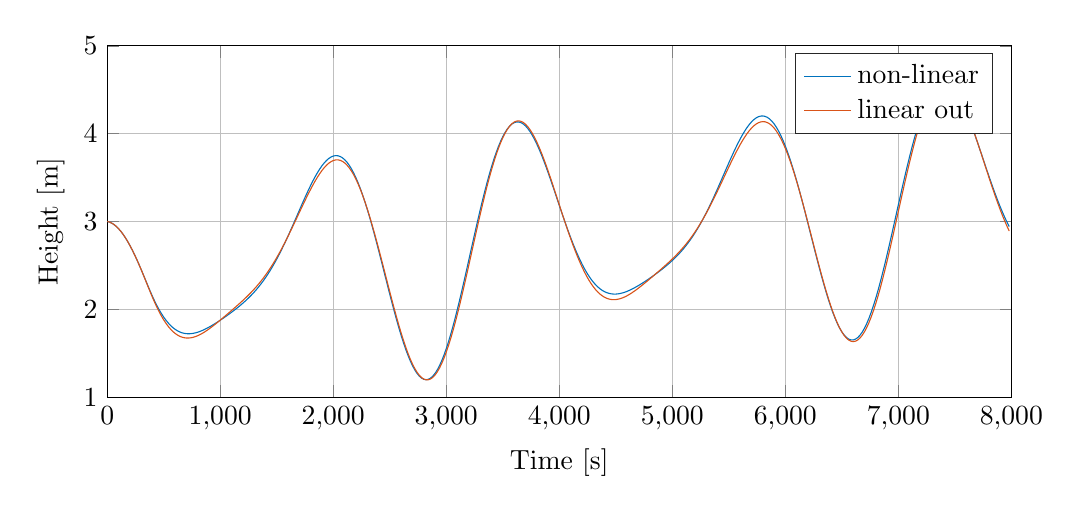
\begin{tikzpicture}

\begin{axis}[%
width=4.521in,
height=1.7566in,
at={(0.758in,0.481in)},
scale only axis,
xmin=0,
xmax=8000,
xlabel={Time [s]},
xmajorgrids,
ymin=1,
ymax=5,
ylabel={Height [m]},
ymajorgrids,
axis background/.style={fill=white},
legend style={legend cell align=left,align=left,draw=white!15!black}
]
\addplot [color=mycolor1,solid]
  table[row sep=crcr]{%
1	3\\
21	2.99281485388517\\
41	2.98089229877703\\
61	2.96429589132252\\
81	2.94311008270548\\
101	2.9174396709271\\
121	2.88740933874452\\
141	2.85316315177336\\
161	2.8148639575681\\
181	2.77269282398572\\
201	2.72684889042081\\
221	2.67755065665281\\
241	2.62504105449041\\
261	2.5696005464303\\
281	2.51157362705104\\
301	2.45141144588331\\
321	2.38972356923401\\
341	2.32731608105155\\
361	2.26518111636098\\
381	2.2044108927358\\
401	2.14604576423477\\
421	2.09091382444387\\
441	2.03953947939103\\
461	1.99216249068991\\
481	1.94883886540228\\
501	1.90955004501104\\
521	1.87426349888611\\
541	1.84294057056688\\
561	1.81552254385374\\
581	1.79192172269374\\
601	1.77202273780071\\
621	1.75568753538331\\
641	1.74275934933769\\
661	1.73306550701636\\
681	1.72642002404801\\
701	1.7226263004337\\
721	1.721480030925\\
741	1.72277250340294\\
761	1.72629422820897\\
781	1.73183850050269\\
801	1.73920436582854\\
821	1.74819864496649\\
841	1.75863713331165\\
861	1.77034559360359\\
881	1.78316126249621\\
901	1.79693507834779\\
921	1.81153406592424\\
941	1.82684296727721\\
961	1.84276464376228\\
981	1.85921963629096\\
1001	1.87614577439579\\
1021	1.89349839419222\\
1041	1.9112509080306\\
1061	1.92939501856447\\
1081	1.94794023088455\\
1101	1.96691302199623\\
1121	1.98635624386529\\
1141	2.00632882547801\\
1161	2.02690520531904\\
1181	2.04817389602818\\
1201	2.07023519122016\\
1221	2.09319861981232\\
1241	2.11718075741644\\
1261	2.14230349649008\\
1281	2.16869239003441\\
1301	2.19647461466528\\
1321	2.22577637273701\\
1341	2.25671984415372\\
1361	2.2894199100356\\
1381	2.32398082346616\\
1401	2.36049293358475\\
1421	2.39902953270337\\
1441	2.43964384317141\\
1461	2.48236609429393\\
1481	2.52720065628709\\
1501	2.57412333151374\\
1521	2.62307902718105\\
1541	2.67397999982164\\
1561	2.72670475185107\\
1581	2.78109761382962\\
1601	2.83696896063655\\
1621	2.89409575718629\\
1641	2.95222200549035\\
1661	3.01105910335552\\
1681	3.07028686578493\\
1701	3.12955608783606\\
1721	3.1884926606673\\
1741	3.24670223308934\\
1761	3.30377434609423\\
1781	3.35928584615839\\
1801	3.41280416341873\\
1821	3.46389102935742\\
1841	3.51210677272424\\
1861	3.55701510759308\\
1881	3.59818829745396\\
1901	3.63521239763498\\
1921	3.6676920072518\\
1941	3.69525411016837\\
1961	3.71755122079759\\
1981	3.73426458404141\\
2001	3.74510796834544\\
2021	3.74983177907082\\
2041	3.74822662577377\\
2061	3.74012575634822\\
2081	3.72540659827193\\
2101	3.70399209968418\\
2121	3.67585224071647\\
2141	3.64100547829182\\
2161	3.59951966604376\\
2181	3.55151220026104\\
2201	3.49714942529824\\
2221	3.4366455543213\\
2241	3.37026156141339\\
2261	3.29830445757568\\
2281	3.22112683622518\\
2301	3.1391259496082\\
2321	3.05274162707454\\
2341	2.96245314986437\\
2361	2.86877586403452\\
2381	2.77225809151969\\
2401	2.67347814098661\\
2421	2.5730408632071\\
2441	2.47157357762109\\
2461	2.36972177433085\\
2481	2.26814510830234\\
2501	2.16751377040952\\
2521	2.06850479198893\\
2541	1.97179767000619\\
2561	1.87806904527067\\
2581	1.78798673595143\\
2601	1.70220377275245\\
2621	1.62135287500041\\
2641	1.54604127573687\\
2661	1.47684551696406\\
2681	1.41430610078412\\
2701	1.35892230840736\\
2721	1.31114754917323\\
2741	1.27138521857775\\
2761	1.2399846969867\\
2781	1.21723718889125\\
2801	1.20337156594245\\
2821	1.19855089642626\\
2841	1.20287042834939\\
2861	1.2163571633426\\
2881	1.23897024873761\\
2901	1.27060120691742\\
2921	1.31107391501638\\
2941	1.36014531158305\\
2961	1.41750773352706\\
2981	1.48279260591013\\
3001	1.55557438301653\\
3021	1.6353741783311\\
3041	1.72166360764023\\
3061	1.81386951256678\\
3081	1.91137934740276\\
3101	2.01354645559838\\
3121	2.11969502354505\\
3141	2.22912531684563\\
3161	2.3411197113053\\
3181	2.45494916084041\\
3201	2.56987928396506\\
3221	2.68517568328921\\
3241	2.8001087923494\\
3261	2.913958718315\\
3281	3.02602030759564\\
3301	3.1356084076647\\
3321	3.24206311786446\\
3341	3.34475464754931\\
3361	3.44308740530391\\
3381	3.5365032781363\\
3401	3.62448442060915\\
3421	3.70655590550318\\
3441	3.78228835741548\\
3461	3.85130050434096\\
3481	3.91326151567244\\
3501	3.96789293803832\\
3521	4.01497001917251\\
3541	4.05432234233896\\
3561	4.08583391781239\\
3581	4.10944298478154\\
3601	4.12514169009504\\
3621	4.13297565675504\\
3641	4.13304336672014\\
3661	4.12549526107345\\
3681	4.11053245796529\\
3701	4.08840500259913\\
3721	4.05940960387706\\
3741	4.02388686315411\\
3761	3.98221805570749\\
3781	3.93482157750421\\
3801	3.88214913282223\\
3821	3.8246816194037\\
3841	3.76292462498394\\
3861	3.69740367134432\\
3881	3.62865958773718\\
3901	3.55724421571929\\
3921	3.48371602283685\\
3941	3.40863487516368\\
3961	3.33255578283922\\
3981	3.25602249087664\\
4001	3.17956215372526\\
4021	3.10368148471852\\
4041	3.02886356459553\\
4061	2.95556421301237\\
4081	2.88420768485663\\
4101	2.81518243063443\\
4121	2.74883781460426\\
4141	2.68548213274398\\
4161	2.62538175049055\\
4181	2.56876106489736\\
4201	2.51580307683372\\
4221	2.46665033670343\\
4241	2.42140592273802\\
4261	2.38013419185734\\
4281	2.34286144601899\\
4301	2.30957709630771\\
4321	2.28023588556642\\
4341	2.2547611701311\\
4361	2.23304871630656\\
4381	2.21497045473843\\
4401	2.20037797896109\\
4421	2.18910577929613\\
4441	2.18097416834298\\
4461	2.17579192958097\\
4481	2.17335895018597\\
4501	2.1734691638205\\
4521	2.17591383375378\\
4541	2.18048485884105\\
4561	2.18697772351799\\
4581	2.19519396597629\\
4601	2.20494328677988\\
4621	2.21604546709222\\
4641	2.22833215082569\\
4661	2.24164844456063\\
4681	2.25585428836781\\
4701	2.2708255958748\\
4721	2.28645518348848\\
4741	2.30265350245163\\
4761	2.31934917075967\\
4781	2.3364892786261\\
4801	2.35403943284029\\
4821	2.37198353486955\\
4841	2.39032332250237\\
4861	2.40907771315782\\
4881	2.42828202071984\\
4901	2.44798719456635\\
4921	2.46825918624809\\
4941	2.48917826047491\\
4961	2.51083779660073\\
4981	2.53334232075012\\
5001	2.55680511312319\\
5021	2.58134605764458\\
5041	2.60708994445858\\
5061	2.63416463695315\\
5081	2.66269835451625\\
5101	2.69281605396968\\
5121	2.72463573619848\\
5141	2.75826549437988\\
5161	2.79380128555438\\
5181	2.83132466101574\\
5201	2.87089978749623\\
5221	2.91256981045269\\
5241	2.95635318565508\\
5261	3.00224059117054\\
5281	3.05019265414474\\
5301	3.10013837362758\\
5321	3.15197395756877\\
5341	3.20556183096077\\
5361	3.26072980166597\\
5381	3.31727066143945\\
5401	3.37494259593204\\
5421	3.43347055786761\\
5441	3.4925484139359\\
5461	3.55184151533162\\
5481	3.61098946395128\\
5501	3.6696090915148\\
5521	3.72729782543722\\
5541	3.7836375758674\\
5561	3.83819905241586\\
5581	3.8905461603198\\
5601	3.94024012274361\\
5621	3.98684336591363\\
5641	4.02992364045296\\
5661	4.06905878912138\\
5681	4.10384197280769\\
5701	4.13388669200904\\
5721	4.15883115084216\\
5741	4.1783420909747\\
5761	4.19211843001435\\
5781	4.19989467435589\\
5801	4.20144371469021\\
5821	4.19657879550007\\
5841	4.18515500359067\\
5861	4.16707089702466\\
5881	4.14227061835941\\
5901	4.11074624672516\\
5921	4.07253970229527\\
5941	4.02774355092192\\
5961	3.976500576373\\
5981	3.91900260892925\\
6001	3.85548928570734\\
6021	3.78624702339909\\
6041	3.71160795367096\\
6061	3.63194843592336\\
6081	3.54768703916759\\
6101	3.45928216013025\\
6121	3.36722945041096\\
6141	3.27205910094471\\
6161	3.17433299360418\\
6181	3.07464172866356\\
6201	2.97360142104793\\
6221	2.8718500232593\\
6241	2.77004303368506\\
6261	2.66884876671112\\
6281	2.56894353856563\\
6301	2.47100692881346\\
6321	2.37571697028913\\
6341	2.28374510092037\\
6361	2.19575095190952\\
6381	2.11237717351843\\
6401	2.03424429733617\\
6421	1.96194541348527\\
6441	1.89604055127532\\
6461	1.8370510171121\\
6481	1.78545413186163\\
6501	1.74167860754163\\
6521	1.70610043102632\\
6541	1.6790389815835\\
6561	1.6607533166525\\
6581	1.65143887375715\\
6601	1.65122492488131\\
6621	1.6601729231616\\
6641	1.67827566834221\\
6661	1.70545722671898\\
6681	1.7415736611061\\
6701	1.78641457950701\\
6721	1.83970528597009\\
6741	1.90110919557292\\
6761	1.97023035897761\\
6781	2.04661632586601\\
6801	2.12976185098345\\
6821	2.21911380386435\\
6841	2.31407704707843\\
6861	2.41402045105396\\
6881	2.51828226495508\\
6901	2.62617483767411\\
6921	2.73698944557072\\
6941	2.85000194650702\\
6961	2.9644792001478\\
6981	3.07968547733259\\
7001	3.19488807684938\\
7021	3.30936204696074\\
7041	3.42239461749967\\
7061	3.53329005553099\\
7081	3.64137506844773\\
7101	3.74600418794656\\
7121	3.84656440006802\\
7141	3.9424787464616\\
7161	4.03320920737392\\
7181	4.11825939471091\\
7201	4.19717735497747\\
7221	4.26955837603005\\
7241	4.33504743694688\\
7261	4.39334099831333\\
7281	4.44418811038861\\
7301	4.48739106335576\\
7321	4.52280583289641\\
7341	4.55034243023618\\
7361	4.56996511018822\\
7381	4.58169230986141\\
7401	4.58559619318552\\
7421	4.58180176312851\\
7441	4.57048560428043\\
7461	4.55187428444757\\
7481	4.5262422751913\\
7501	4.49390920767586\\
7521	4.45523654501246\\
7541	4.41062407828374\\
7561	4.3605065875251\\
7581	4.3053505303558\\
7601	4.24565025018577\\
7621	4.18192336124105\\
7641	4.1147054943826\\
7661	4.04454491654018\\
7681	3.97199740362714\\
7701	3.89762137691474\\
7721	3.82197307044025\\
7741	3.74560152687094\\
7761	3.66904342647833\\
7781	3.59281791356527\\
7801	3.51742161190686\\
7821	3.4433240170121\\
7841	3.37096350522146\\
7861	3.30074415787586\\
7881	3.23303334381679\\
7901	3.16815978792106\\
7921	3.10641197774448\\
7941	3.04803704469674\\
7961	2.99324029031497\\
7981	2.9421853164876\\
};
\addlegendentry{non-linear};

\addplot [color=mycolor2,solid]
  table[row sep=crcr]{%
1	3\\
21	2.99281440022489\\
41	2.98089141779219\\
61	2.96429466742038\\
81	2.94310852843827\\
101	2.91743776991418\\
121	2.88740708529663\\
141	2.85316053936219\\
161	2.81486093459038\\
181	2.77268912386595\\
201	2.72684337432509\\
221	2.67753913883185\\
241	2.62501024463012\\
261	2.56951382086477\\
281	2.51134312777761\\
301	2.45085350061734\\
321	2.38850389609367\\
341	2.32490689651401\\
361	2.26086469593234\\
381	2.19735754551971\\
401	2.13546001054403\\
421	2.07619581325621\\
441	2.02038619729244\\
461	1.96856310452994\\
481	1.92098453239321\\
501	1.87772649565134\\
521	1.83878562469752\\
541	1.80413966256706\\
561	1.77375918889231\\
581	1.74759670755254\\
601	1.72557777749333\\
621	1.70760023833348\\
641	1.69353634121097\\
661	1.68323383516125\\
681	1.67651651959424\\
701	1.67318610518368\\
721	1.67302626683397\\
741	1.67580860489385\\
761	1.68129925675633\\
781	1.68926430156763\\
801	1.69947246429996\\
821	1.71169505786083\\
841	1.72570486204734\\
861	1.74127655481244\\
881	1.75819046115501\\
901	1.77623896485616\\
921	1.79523262762844\\
941	1.81500293195674\\
961	1.83540102240988\\
981	1.85629489650047\\
1001	1.87756846491075\\
1021	1.89912388894067\\
1041	1.92088556786785\\
1061	1.94280300432016\\
1081	1.96485137684611\\
1101	1.98703091082509\\
1121	2.00936646239014\\
1141	2.03190700860737\\
1161	2.05472336566124\\
1181	2.07790336305972\\
1201	2.10154602873364\\
1221	2.12575749555886\\
1241	2.15065000183501\\
1261	2.17634284530286\\
1281	2.20296280112521\\
1301	2.23064225139466\\
1321	2.25951504816445\\
1341	2.28971136351562\\
1361	2.32135283865976\\
1381	2.35454868962405\\
1401	2.38939277948566\\
1421	2.42596133177235\\
1441	2.46431086503161\\
1461	2.50447601865764\\
1481	2.54646726337093\\
1501	2.59026890339358\\
1521	2.63583788243815\\
1541	2.68310352483084\\
1561	2.73196783839336\\
1581	2.78230579374976\\
1601	2.83396500514502\\
1621	2.88676433312902\\
1641	2.94049151036878\\
1661	2.99490120017349\\
1681	3.04971584458331\\
1701	3.1046305830461\\
1721	3.15932060281873\\
1741	3.2134471626389\\
1761	3.26665957414212\\
1781	3.31859380658489\\
1801	3.36887088799438\\
1821	3.41709790756111\\
1841	3.46287225353468\\
1861	3.50578800782363\\
1881	3.54544293830718\\
1901	3.58144458644417\\
1921	3.61341423281511\\
1941	3.64098856354527\\
1961	3.66382055133951\\
1981	3.68158195460237\\
2001	3.69396863639902\\
2021	3.70070734279292\\
2041	3.70156106983967\\
2061	3.69633130076715\\
2081	3.68485811011808\\
2101	3.66702064224112\\
2121	3.64273938010825\\
2141	3.61197937354622\\
2161	3.57475261278412\\
2181	3.53111867734245\\
2201	3.48118434790364\\
2221	3.42510366270219\\
2241	3.3630795742928\\
2261	3.29536708433595\\
2281	3.22227601516605\\
2301	3.14417076185021\\
2321	3.06146578977252\\
2341	2.97461854542215\\
2361	2.88412302122661\\
2381	2.79050578668944\\
2401	2.69432359996626\\
2421	2.59616078158069\\
2441	2.49662595586482\\
2461	2.39634928376956\\
2481	2.29598089223822\\
2501	2.19618937416538\\
2521	2.09765812683753\\
2541	2.00107821425157\\
2561	1.90713867994491\\
2581	1.81651692743442\\
2601	1.72987153220216\\
2621	1.64783790317654\\
2641	1.5710253008542\\
2661	1.50001348075788\\
2681	1.43534853860873\\
2701	1.37753866771737\\
2721	1.32705024922676\\
2741	1.28430363838373\\
2761	1.2496677582803\\
2781	1.2234537120066\\
2801	1.20590910720385\\
2821	1.19721522934085\\
2841	1.19748789352765\\
2861	1.20678041583414\\
2881	1.22508562613702\\
2901	1.25233496368744\\
2921	1.28839587223512\\
2941	1.33307086495155\\
2961	1.38610029478373\\
2981	1.4471673430214\\
3001	1.51590197071301\\
3021	1.59188249129099\\
3041	1.67463650867943\\
3061	1.7636434802498\\
3081	1.85833891581711\\
3101	1.958118551448\\
3121	2.06234190664612\\
3141	2.17033661028885\\
3161	2.28140474143919\\
3181	2.3948302344061\\
3201	2.50988507431779\\
3221	2.62583329838828\\
3241	2.74193413290112\\
3261	2.85744637870939\\
3281	2.97163497153952\\
3301	3.08377900167909\\
3321	3.19317961121229\\
3341	3.29916622491028\\
3361	3.40110036059106\\
3381	3.49837759373784\\
3401	3.59042931857685\\
3421	3.67672581514473\\
3441	3.75678091338381\\
3461	3.8301573464424\\
3481	3.89647148484589\\
3501	3.95539642949017\\
3521	4.00666307884176\\
3541	4.05005961530232\\
3561	4.08543054189667\\
3581	4.1126764197232\\
3601	4.1317547263438\\
3621	4.14268135230373\\
3641	4.14553179778543\\
3661	4.14044122600704\\
3681	4.12760290734496\\
3701	4.10726502192496\\
3721	4.07972617798186\\
3741	4.04533026238728\\
3761	4.00446129512958\\
3781	3.95753878429585\\
3801	3.90501370702604\\
3821	3.84736489230623\\
3841	3.78509560617983\\
3861	3.71873049121387\\
3881	3.64881295666393\\
3901	3.57590217284673\\
3921	3.50056794795699\\
3941	3.42338262448818\\
3961	3.34491172325763\\
3981	3.26570688799794\\
4001	3.18630329792636\\
4021	3.10721992864316\\
4041	3.02895855698105\\
4061	2.95199883335327\\
4081	2.87679063443408\\
4101	2.80374741778049\\
4121	2.73324340066727\\
4141	2.66561456771732\\
4161	2.60116150102129\\
4181	2.54015188755756\\
4201	2.48282142453608\\
4221	2.42937263359204\\
4241	2.37997167114148\\
4261	2.33474399765706\\
4281	2.2937707314359\\
4301	2.25708787779384\\
4321	2.22468957385159\\
4341	2.1965343574163\\
4361	2.1725518665718\\
4381	2.15264762666721\\
4401	2.13670521975603\\
4421	2.12458656151609\\
4441	2.11613144767592\\
4461	2.11115749989987\\
4481	2.10946161485236\\
4501	2.11082361718534\\
4521	2.11501173176686\\
4541	2.12178841931948\\
4561	2.1309150739812\\
4581	2.1421551022387\\
4601	2.15527600182056\\
4621	2.17005135124518\\
4641	2.18626314912038\\
4661	2.2037043768516\\
4681	2.22218147653031\\
4701	2.24151656679536\\
4721	2.26154935663942\\
4741	2.28213872621155\\
4761	2.30316389783505\\
4781	2.32452511666079\\
4801	2.34614384105002\\
4821	2.36796259414572\\
4841	2.38994475580475\\
4861	2.41207457635342\\
4881	2.43435757420532\\
4901	2.45682123996896\\
4921	2.47951551657257\\
4941	2.50251203777455\\
4961	2.52590130124138\\
4981	2.54978824073636\\
5001	2.57428802776176\\
5021	2.59952362744324\\
5041	2.625624528274\\
5061	2.65272443625514\\
5081	2.68095671801529\\
5101	2.71044911073355\\
5121	2.7413205085844\\
5141	2.77368078022732\\
5161	2.80763146790028\\
5181	2.84326419708684\\
5201	2.88065568918607\\
5221	2.91986120300855\\
5241	2.96090928549777\\
5261	3.00379938910524\\
5281	3.04850185780044\\
5301	3.09495866567559\\
5321	3.14308348860742\\
5341	3.19276067453259\\
5361	3.24384377647537\\
5381	3.29615489914353\\
5401	3.34948576206428\\
5421	3.40360030578504\\
5441	3.45823772372026\\
5461	3.51311476615719\\
5481	3.56792698393648\\
5501	3.62234949702098\\
5521	3.67603818144276\\
5541	3.72863175213521\\
5561	3.77975448997064\\
5581	3.82901893025311\\
5601	3.87602817095107\\
5621	3.92037845227339\\
5641	3.96166334842342\\
5661	3.99948025008013\\
5681	4.03343804471769\\
5701	4.06316372222427\\
5721	4.08830637759624\\
5741	4.10853899315422\\
5761	4.12355943533883\\
5781	4.13309149249345\\
5801	4.13688581717754\\
5821	4.13472086083748\\
5841	4.12640498792909\\
5861	4.11178120763315\\
5881	4.0907344805728\\
5901	4.06319942169946\\
5921	4.02916531532821\\
5941	3.98867658795233\\
5961	3.94182946966311\\
5981	3.88876764871447\\
6001	3.82967971438443\\
6021	3.76479919195388\\
6041	3.69440582897694\\
6061	3.61882629787133\\
6081	3.53843361290349\\
6101	3.45364577375702\\
6121	3.36492430478756\\
6141	3.27277276432509\\
6161	3.17773481406127\\
6181	3.08039131534318\\
6201	2.98135595117596\\
6221	2.88126915388447\\
6241	2.78079086369663\\
6261	2.68059340135463\\
6281	2.58135561607663\\
6301	2.48375838843652\\
6321	2.38848061716221\\
6341	2.29619492786121\\
6361	2.20756306607149\\
6381	2.12323116120915\\
6401	2.0438246002971\\
6421	1.96994208360107\\
6441	1.90214913581489\\
6461	1.84097217388209\\
6481	1.7868940691457\\
6501	1.74035100857542\\
6521	1.70172953772122\\
6541	1.67136290511889\\
6561	1.649526931844\\
6581	1.63643648119307\\
6601	1.6322434391256\\
6621	1.63703623204657\\
6641	1.65084024245426\\
6661	1.67361854510173\\
6681	1.70527275956482\\
6701	1.74564385343696\\
6721	1.79451250649017\\
6741	1.85159881399067\\
6761	1.91656190886006\\
6781	1.98900090127534\\
6801	2.06845848653744\\
6821	2.15442733725718\\
6841	2.24635761710874\\
6861	2.3436630296927\\
6881	2.44572388379015\\
6901	2.55188821702711\\
6921	2.66147387383335\\
6941	2.77377371349836\\
6961	2.88806341135564\\
6981	3.00360919293304\\
7001	3.11967326778472\\
7021	3.235517179709\\
7041	3.35040540902431\\
7061	3.4636113984983\\
7081	3.5744259000194\\
7101	3.68216526811965\\
7121	3.78617714678074\\
7141	3.88584299178917\\
7161	3.98057913735402\\
7181	4.06983871503306\\
7201	4.15311543798356\\
7221	4.22994843693838\\
7241	4.29992648767778\\
7261	4.36269056814456\\
7281	4.41793501103677\\
7301	4.46540841658513\\
7321	4.50491532472236\\
7341	4.53631873616528\\
7361	4.55954273946846\\
7381	4.57457427509407\\
7401	4.58146340342134\\
7421	4.58032198896795\\
7441	4.57132108096684\\
7461	4.55468725231449\\
7481	4.5306979976484\\
7501	4.49967651581627\\
7521	4.46198680804613\\
7541	4.41803013333666\\
7561	4.36824280717216\\
7581	4.31309388842915\\
7601	4.25308109499283\\
7621	4.1887247748573\\
7641	4.12056147131979\\
7661	4.04913882264298\\
7681	3.97501216300889\\
7701	3.8987417055821\\
7721	3.82088886078933\\
7741	3.74201106822952\\
7761	3.66265561022345\\
7781	3.58335342431708\\
7801	3.50461380895877\\
7821	3.42692052917991\\
7841	3.35072947163008\\
7861	3.27646753590179\\
7881	3.20453188365312\\
7901	3.1352885687198\\
7921	3.06907030219124\\
7941	3.00617398347174\\
7961	2.94685869728292\\
7981	2.89134426856577\\
};
\addlegendentry{linear out};

\end{axis}
\end{tikzpicture}%
\caption{Comparison of the nonlinear and linear model for the tank. }
\label{fig:linear_nonlinear_comparison_tank_height}
\end{figure}
 
It is clear that the nonlinear and linear model for the tank are very similar as they only deviate a small amount at the peaks. In figure \ref{fig:linear_nonlinear_comparison_pipe_after_tank} the output of the pipe after the tank is shown.  

\begin{figure}[H]
 \centering
 % This file was created by matlab2tikz.
%
%The latest updates can be retrieved from
%  http://www.mathworks.com/matlabcentral/fileexchange/22022-matlab2tikz-matlab2tikz
%where you can also make suggestions and rate matlab2tikz.
%
\definecolor{mycolor1}{rgb}{0.00000,0.44700,0.74100}%
\definecolor{mycolor2}{rgb}{0.85000,0.32500,0.09800}%
%
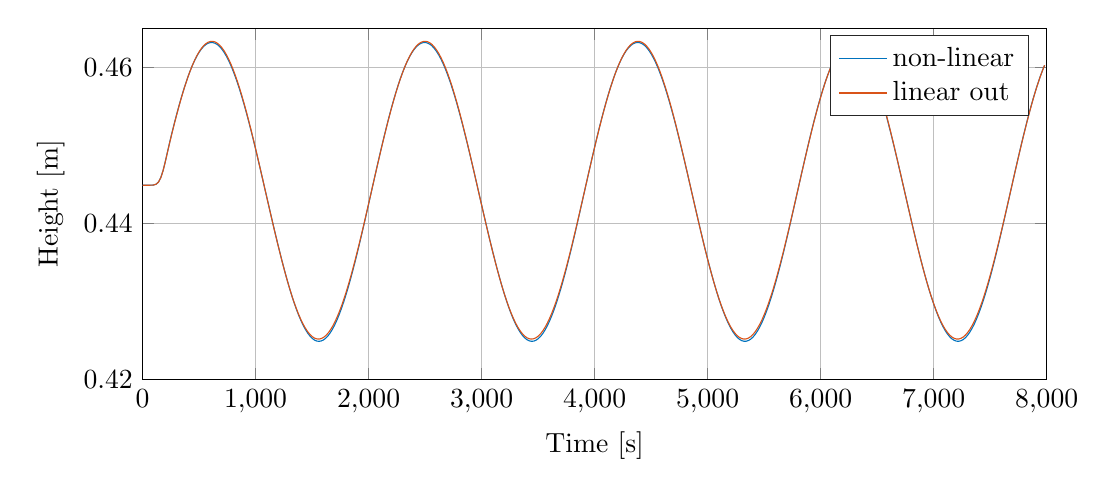
\begin{tikzpicture}

\begin{axis}[%
width=4.521in,
height=1.7566in,
at={(0.758in,0.481in)},
scale only axis,
xmin=0,
xmax=8000,
xlabel={Time [s]},
xmajorgrids,
ymin=0.42,
ymax=0.465,
ylabel={Height [m]},
ymajorgrids,
axis background/.style={fill=white},
legend style={legend cell align=left,align=left,draw=white!15!black}
]
\addplot [color=mycolor1,solid]
  table[row sep=crcr]{%
1	0.4448903921446\\
21	0.444890395604401\\
41	0.444890478989189\\
61	0.444891399462415\\
81	0.44489768087895\\
101	0.444927316973418\\
121	0.445029837966795\\
141	0.445299119740533\\
161	0.445848740544978\\
181	0.446737111169511\\
201	0.447900409457629\\
221	0.449181948114068\\
241	0.450445971436173\\
261	0.451649238232275\\
281	0.452805509195267\\
301	0.453923614919199\\
321	0.454996760490511\\
341	0.456018473924374\\
361	0.456985842499905\\
381	0.457895758609179\\
401	0.458744309155889\\
421	0.459526872446132\\
441	0.460238927080553\\
461	0.460877766766091\\
481	0.461442404335922\\
501	0.461931618263264\\
521	0.462343038226796\\
541	0.462673985796383\\
561	0.462922115566296\\
581	0.463085761808448\\
601	0.463165000862207\\
621	0.463161767963357\\
641	0.463077774152749\\
661	0.462912700515528\\
681	0.462665083217703\\
701	0.462334975525558\\
721	0.461925320066751\\
741	0.461439882474596\\
761	0.46088032121217\\
781	0.460247109256119\\
801	0.459542826148449\\
821	0.45877213118035\\
841	0.457938885851068\\
861	0.457045736413618\\
881	0.456096249484013\\
901	0.455095257701042\\
921	0.454047285512727\\
941	0.45295630118541\\
961	0.451826616747197\\
981	0.450662864559418\\
1001	0.449469684812144\\
1021	0.448252115056624\\
1041	0.447015762927058\\
1061	0.445766484480015\\
1081	0.444510082772652\\
1101	0.443251681187692\\
1121	0.441995298599495\\
1141	0.440745148396479\\
1161	0.439507469163443\\
1181	0.438289725378601\\
1201	0.437097776851792\\
1221	0.435935185912507\\
1241	0.434805514793038\\
1261	0.433713925442494\\
1281	0.432666274604885\\
1301	0.43166800385088\\
1321	0.430724234156608\\
1341	0.429839588257958\\
1361	0.429017425169056\\
1381	0.428260320657075\\
1401	0.427571617572048\\
1421	0.426955499857992\\
1441	0.426415400429793\\
1461	0.425953448340526\\
1481	0.425571672054113\\
1501	0.425272672419593\\
1521	0.425058857459238\\
1541	0.424931824128951\\
1561	0.424892442284851\\
1581	0.424940683805082\\
1601	0.425075517272546\\
1621	0.425295832195707\\
1641	0.425601309173907\\
1661	0.42599160714887\\
1681	0.426465142574227\\
1701	0.427019705714707\\
1721	0.427653493342147\\
1741	0.428363981002374\\
1761	0.42914653153053\\
1781	0.429995804679556\\
1801	0.430908099193119\\
1821	0.431881059821401\\
1841	0.432911394765246\\
1861	0.433993705632748\\
1881	0.435121373864266\\
1901	0.436288299080676\\
1921	0.437489773956437\\
1941	0.43872116706734\\
1961	0.439976132856488\\
1981	0.441247642314717\\
2001	0.442530281676256\\
2021	0.443819748072584\\
2041	0.445110556898724\\
2061	0.446395579129906\\
2081	0.447667614489687\\
2101	0.448920774822279\\
2121	0.450150357835776\\
2141	0.451351868388035\\
2161	0.452520326999804\\
2181	0.453650018421382\\
2201	0.454735047647489\\
2221	0.455770604767913\\
2241	0.456752920117414\\
2261	0.45767786232995\\
2281	0.458540886029431\\
2301	0.459338220671602\\
2321	0.460067093113085\\
2341	0.460725078416789\\
2361	0.461309562370026\\
2381	0.461817806407534\\
2401	0.462247763273825\\
2421	0.462598216405697\\
2441	0.462867637999104\\
2461	0.463053931290156\\
2481	0.463155758716082\\
2501	0.463173406987413\\
2521	0.463108216873153\\
2541	0.462961344264138\\
2561	0.462733016609565\\
2581	0.462423290393124\\
2601	0.462033536184375\\
2621	0.461566468741214\\
2641	0.461024587561179\\
2661	0.460409429076971\\
2681	0.45972289769997\\
2701	0.458968673915622\\
2721	0.458151234210152\\
2741	0.457273755204186\\
2761	0.456338405360126\\
2781	0.455348784584706\\
2801	0.454310509462161\\
2821	0.453229024500086\\
2841	0.45210834751631\\
2861	0.450952377431298\\
2881	0.449766047548192\\
2901	0.448554934220683\\
2921	0.447324583029557\\
2941	0.446079816050748\\
2961	0.444824516575756\\
2981	0.443563280683107\\
3001	0.442302896370496\\
3021	0.441050635562948\\
3041	0.439811829783472\\
3061	0.438590491144546\\
3081	0.437391337729156\\
3101	0.43621999467303\\
3121	0.43508187855787\\
3141	0.433981766139539\\
3161	0.432924180977651\\
3181	0.431913798138767\\
3201	0.430955501332743\\
3221	0.430053967465686\\
3241	0.429213319660685\\
3261	0.428437532100341\\
3281	0.427730857251183\\
3301	0.427097346371492\\
3321	0.426540012552986\\
3341	0.426060609240445\\
3361	0.425660424927357\\
3381	0.42534150905032\\
3401	0.425106742198916\\
3421	0.424958354230932\\
3441	0.424896842830342\\
3461	0.424921822321892\\
3481	0.425033402317752\\
3501	0.425231955647634\\
3521	0.42551694416182\\
3541	0.425886728089751\\
3561	0.42633940220955\\
3581	0.426873588121702\\
3601	0.427488068486536\\
3621	0.428180163988864\\
3641	0.428945260426252\\
3661	0.429778734242722\\
3681	0.430677124447792\\
3701	0.431636789703454\\
3721	0.432653169289003\\
3741	0.433721738054433\\
3761	0.434837739429171\\
3781	0.435995142723564\\
3801	0.437187842171712\\
3821	0.438411292119205\\
3841	0.439661292849863\\
3861	0.440931906439047\\
3881	0.442215624625787\\
3901	0.44350503171859\\
3921	0.444794047103543\\
3941	0.446078036731297\\
3961	0.447352680571852\\
3981	0.448612377739923\\
4001	0.449850008919513\\
4021	0.451058754686546\\
4041	0.452233722383858\\
4061	0.453371231444124\\
4081	0.45446718661151\\
4101	0.455516626164891\\
4121	0.45651413073549\\
4141	0.457454417368793\\
4161	0.458333032126385\\
4181	0.459146554164511\\
4201	0.459892187563285\\
4221	0.460567574708783\\
4241	0.461170767662515\\
4261	0.46169945399006\\
4281	0.462150296522625\\
4301	0.462520073624152\\
4321	0.462807419534523\\
4341	0.463012672428474\\
4361	0.463136209934371\\
4381	0.463177453834328\\
4401	0.463135364993678\\
4421	0.463009448734659\\
4441	0.462800168055425\\
4461	0.462508899904114\\
4481	0.462137766580776\\
4501	0.461689079894435\\
4521	0.461164903287343\\
4541	0.460567387576779\\
4561	0.459899027091285\\
4581	0.459162323214267\\
4601	0.458359914215142\\
4621	0.457495281171775\\
4641	0.456572841030437\\
4661	0.455597256182129\\
4681	0.454572625454353\\
4701	0.45350233087259\\
4721	0.452390243485219\\
4741	0.451241869978709\\
4761	0.450063157636792\\
4781	0.448858575481812\\
4801	0.447631852097398\\
4821	0.446388216864328\\
4841	0.445134364231608\\
4861	0.443876196685799\\
4881	0.442617808206113\\
4901	0.441363085332201\\
4921	0.44011758302659\\
4941	0.43888829668457\\
4961	0.437682050968897\\
4981	0.436504430852266\\
5001	0.435359509464875\\
5021	0.434250382592523\\
5041	0.433180992539732\\
5061	0.432157373823571\\
5081	0.431185984086408\\
5101	0.4302713617276\\
5121	0.429416716996079\\
5141	0.428625937154064\\
5161	0.427903290324115\\
5181	0.427251705466141\\
5201	0.42667322348645\\
5221	0.426171009347273\\
5241	0.425749077659214\\
5261	0.425410139678574\\
5281	0.425155495681146\\
5301	0.424986496922649\\
5321	0.424904161966396\\
5341	0.4249081147041\\
5361	0.424997774028669\\
5381	0.42517394614022\\
5401	0.425437656708292\\
5421	0.425787756900242\\
5441	0.426221178786418\\
5461	0.426735542295589\\
5481	0.427329902935067\\
5501	0.428002586084727\\
5521	0.428749624735279\\
5541	0.429565913543407\\
5561	0.430447358222041\\
5581	0.431391281066433\\
5601	0.432394554664011\\
5621	0.433452109331753\\
5641	0.434557897475042\\
5661	0.435706370015107\\
5681	0.436892151527985\\
5701	0.438109231903986\\
5721	0.439351542835237\\
5741	0.44061391847583\\
5761	0.4418917791553\\
5781	0.443179972659237\\
5801	0.444472112203118\\
5821	0.445760901135628\\
5841	0.447039410431999\\
5861	0.448302294640601\\
5881	0.449545070145216\\
5901	0.450762244389867\\
5921	0.451947439561802\\
5941	0.453095196214922\\
5961	0.454201225542087\\
5981	0.455261167747205\\
6001	0.456270449575444\\
6021	0.457225032424042\\
6041	0.458120965883983\\
6061	0.458953405335724\\
6081	0.459717398106615\\
6101	0.460409784421205\\
6121	0.461029393598847\\
6141	0.461575226284475\\
6161	0.46204506531963\\
6181	0.462435806943492\\
6201	0.462744755541305\\
6221	0.462970831698769\\
6241	0.463114316881196\\
6261	0.46317502160788\\
6281	0.463151889874882\\
6301	0.463044937140545\\
6321	0.462855668457809\\
6341	0.462585317371394\\
6361	0.462234832468149\\
6381	0.461806333185606\\
6401	0.461302476892736\\
6421	0.460724749910288\\
6441	0.460073913949511\\
6461	0.459352032782993\\
6481	0.458563403729106\\
6501	0.457713431193128\\
6521	0.456806556288546\\
6541	0.455845440203154\\
6561	0.45483259924341\\
6581	0.453772376411493\\
6601	0.452670257986183\\
6621	0.451530831792248\\
6641	0.450358104364117\\
6661	0.449157481130739\\
6681	0.447935492522085\\
6701	0.446697427736366\\
6721	0.445446756387308\\
6741	0.444187416285592\\
6761	0.442925813114962\\
6781	0.441669557344039\\
6801	0.440424493889265\\
6821	0.439194336992158\\
6841	0.437983117309509\\
6861	0.436796437622876\\
6881	0.43564025171452\\
6901	0.434519651366974\\
6921	0.433439380042675\\
6941	0.432404876126699\\
6961	0.431421641971086\\
6981	0.430493757393094\\
7001	0.429624388855023\\
7021	0.428817301676938\\
7041	0.428076463269876\\
7061	0.427405277647129\\
7081	0.426807433424893\\
7101	0.426286817103075\\
7121	0.425845962322018\\
7141	0.425486547435813\\
7161	0.425210959859231\\
7181	0.42502117763164\\
7201	0.424917303859516\\
7221	0.424899039023663\\
7241	0.42496709997489\\
7261	0.425122169566122\\
7281	0.425363956731929\\
7301	0.42569169491415\\
7321	0.426104376292536\\
7341	0.42660020218337\\
7361	0.42717636956689\\
7381	0.427829719381899\\
7401	0.428557433919051\\
7421	0.429356686575398\\
7441	0.430223719155471\\
7461	0.43115382378206\\
7481	0.432142239450521\\
7501	0.433184761575379\\
7521	0.434277436478473\\
7541	0.435415577258436\\
7561	0.436593187205938\\
7581	0.437803755423473\\
7601	0.439041525793268\\
7621	0.440301526199249\\
7641	0.441578252590158\\
7661	0.442864799055158\\
7681	0.444154054094442\\
7701	0.445440665631803\\
7721	0.446720763362201\\
7741	0.447989443517319\\
7761	0.44923954601381\\
7781	0.450463741546056\\
7801	0.451656945962332\\
7821	0.45281528223829\\
7841	0.453933601970715\\
7861	0.45500586124484\\
7881	0.456027171155159\\
7901	0.456994075124528\\
7921	0.457903412207435\\
7941	0.458751392878064\\
7961	0.45953334892597\\
7981	0.460244767047644\\
};
\addlegendentry{non-linear};

\addplot [color=mycolor2,solid]
  table[row sep=crcr]{%
1	0.4448903921446\\
21	0.444890395617133\\
41	0.444890478026722\\
61	0.444891388734201\\
81	0.444897606167967\\
101	0.444926944647608\\
121	0.445028415823967\\
141	0.445294815737426\\
161	0.445838317964045\\
181	0.446716904530933\\
201	0.447868694158873\\
221	0.44914008148068\\
241	0.450396431268791\\
261	0.451593706287482\\
281	0.45274591716805\\
301	0.453863446187736\\
321	0.454940097997123\\
341	0.455968623918073\\
361	0.456944989724898\\
381	0.457865090257204\\
401	0.458724683099225\\
421	0.459519979485693\\
441	0.460247453395949\\
461	0.460903864640065\\
481	0.461486300746845\\
501	0.46199217273643\\
521	0.462419233510585\\
541	0.462765585623977\\
561	0.463029690327448\\
581	0.463210374251882\\
601	0.463306834656033\\
621	0.463318642985552\\
641	0.463245746778447\\
661	0.463088469897877\\
681	0.462847511093349\\
701	0.462523940896301\\
721	0.46211919686395\\
741	0.461635077192516\\
761	0.461073732728197\\
781	0.460437657411391\\
801	0.459729677196624\\
821	0.458952937497402\\
841	0.45811088921177\\
861	0.457207273390672\\
881	0.45624610461721\\
901	0.455231653170664\\
921	0.454168426054497\\
941	0.45306114697265\\
961	0.451914735343076\\
981	0.450734284441755\\
1001	0.449525038774296\\
1021	0.448292370775654\\
1041	0.447041756941486\\
1061	0.445778753497181\\
1081	0.444508971712668\\
1101	0.443238052972682\\
1121	0.441971643713216\\
1141	0.440715370335554\\
1161	0.439474814209296\\
1181	0.438255486875459\\
1201	0.437062805559814\\
1221	0.435902069105237\\
1241	0.434778434430021\\
1261	0.433696893616724\\
1281	0.432662251733357\\
1301	0.431679105485427\\
1321	0.430751822793706\\
1341	0.429884523388436\\
1361	0.4290810605062\\
1381	0.428345003770763\\
1401	0.427679623333958\\
1421	0.427087875347057\\
1441	0.426572388827185\\
1461	0.426135453977131\\
1481	0.425779012010433\\
1501	0.425504646526962\\
1521	0.425313576477302\\
1541	0.425206650747203\\
1561	0.425184344386148\\
1581	0.425246756496807\\
1601	0.425393609794741\\
1621	0.425624251840326\\
1641	0.425937657937404\\
1661	0.426332435685806\\
1681	0.426806831167505\\
1701	0.427358736738922\\
1721	0.427985700394756\\
1741	0.428684936661757\\
1761	0.429453338974018\\
1781	0.430287493474825\\
1801	0.431183694183729\\
1821	0.43213795946148\\
1841	0.433146049699638\\
1861	0.434203486156307\\
1881	0.43530557085428\\
1901	0.436447407453207\\
1921	0.437623923003047\\
1941	0.438829890482165\\
1961	0.440059952019936\\
1981	0.441308642700684\\
2001	0.442570414843205\\
2021	0.443839662647992\\
2041	0.445110747102678\\
2061	0.44637802103503\\
2081	0.4476358542022\\
2101	0.448878658304755\\
2121	0.450100911814371\\
2141	0.45129718450487\\
2161	0.45246216157762\\
2181	0.453590667274116\\
2201	0.454677687870831\\
2221	0.455718393954183\\
2241	0.456708161876644\\
2261	0.457642594298676\\
2281	0.458517539725225\\
2301	0.459329110949977\\
2321	0.460073702325432\\
2341	0.460748005782071\\
2361	0.461349025525443\\
2381	0.461874091345875\\
2401	0.462320870481676\\
2421	0.462687377983128\\
2441	0.462971985531217\\
2461	0.463173428671929\\
2481	0.463290812433959\\
2501	0.463323615304894\\
2521	0.463271691548187\\
2541	0.463135271850629\\
2561	0.462914962297462\\
2581	0.46261174167966\\
2601	0.462226957145359\\
2621	0.461762318214747\\
2641	0.461219889185015\\
2661	0.460602079959095\\
2681	0.459911635338949\\
2701	0.459151622830968\\
2721	0.458325419017657\\
2741	0.457436694556158\\
2761	0.456489397870264\\
2781	0.455487737608361\\
2801	0.454436163945257\\
2821	0.453339348810948\\
2841	0.452202165134174\\
2861	0.45102966519298\\
2881	0.449827058168461\\
2901	0.448599687001419\\
2921	0.447353004654753\\
2941	0.446092549887046\\
2961	0.444823922644971\\
2981	0.443552759183861\\
3001	0.442284707026959\\
3021	0.441025399874608\\
3041	0.439780432574861\\
3061	0.438555336266689\\
3081	0.437355553806254\\
3101	0.436186415585388\\
3121	0.435053115849739\\
3141	0.433960689621784\\
3161	0.432913990331236\\
3181	0.431917668252236\\
3201	0.430976149843119\\
3221	0.430093618080554\\
3241	0.429273993875416\\
3261	0.428520918652976\\
3281	0.427837738174776\\
3301	0.427227487674086\\
3321	0.426692878370975\\
3341	0.426236285426905\\
3361	0.425859737392369\\
3381	0.425564907194445\\
3401	0.425353104704323\\
3421	0.425225270917811\\
3441	0.425181973774675\\
3461	0.425223405635402\\
3481	0.425349382426579\\
3501	0.425559344458695\\
3521	0.425852358912728\\
3541	0.426227123984474\\
3561	0.426681974668195\\
3581	0.427214890153914\\
3601	0.427823502805456\\
3621	0.428505108679388\\
3641	0.429256679538088\\
3661	0.430074876303599\\
3681	0.430956063892478\\
3701	0.431896327365742\\
3721	0.43289148932215\\
3741	0.433937128457557\\
3761	0.435028599207879\\
3781	0.436161052388397\\
3801	0.437329456737708\\
3821	0.438528621270607\\
3841	0.43975321834059\\
3861	0.440997807309512\\
3881	0.442256858719245\\
3901	0.443524778857953\\
3921	0.444795934611821\\
3941	0.446064678491848\\
3961	0.447325373724503\\
3981	0.448572419294775\\
4001	0.449800274830353\\
4021	0.451003485216384\\
4041	0.452176704831453\\
4061	0.453314721297099\\
4081	0.454412478635365\\
4101	0.455465099731487\\
4121	0.456467908001936\\
4141	0.457416448171533\\
4161	0.458306506067343\\
4181	0.459134127341396\\
4201	0.459895635039054\\
4221	0.460587645934987\\
4241	0.461207085564157\\
4261	0.461751201881048\\
4281	0.462217577486449\\
4301	0.462604140367476\\
4321	0.462909173103103\\
4341	0.463131320494319\\
4361	0.463269595585006\\
4381	0.463323384046786\\
4401	0.463292446908355\\
4421	0.463176921617189\\
4441	0.46297732142889\\
4461	0.462694533126894\\
4481	0.462329813082673\\
4501	0.461884781673928\\
4521	0.461361416085577\\
4541	0.460762041525523\\
4561	0.46008932089422\\
4581	0.459346242953946\\
4601	0.458536109050333\\
4621	0.45766251844515\\
4641	0.456729352325514\\
4661	0.455740756560553\\
4681	0.454701123282144\\
4701	0.45361507137156\\
4721	0.452487425938706\\
4741	0.451323196885129\\
4761	0.450127556646036\\
4781	0.448905817210206\\
4801	0.44766340651989\\
4821	0.446405844355561\\
4841	0.445138717812639\\
4861	0.443867656479153\\
4881	0.442598307424612\\
4901	0.441336310111216\\
4921	0.44008727133886\\
4941	0.438856740335249\\
4961	0.437650184101802\\
4981	0.436472963124859\\
5001	0.435330307560128\\
5021	0.434227293996148\\
5041	0.433168822900035\\
5061	0.43215959684569\\
5081	0.431204099621212\\
5101	0.430306576308332\\
5121	0.429471014422363\\
5141	0.428701126196483\\
5161	0.42800033208902\\
5181	0.427371745587054\\
5201	0.426818159373814\\
5221	0.42634203292135\\
5241	0.4259454815636\\
5261	0.425630267098379\\
5281	0.425397789960071\\
5301	0.42524908299778\\
5321	0.42518480688659\\
5341	0.425205247192317\\
5361	0.4253103131028\\
5381	0.425499537831359\\
5401	0.425772080690636\\
5421	0.426126730827597\\
5441	0.42656191260311\\
5461	0.427075692592195\\
5481	0.427665788173836\\
5501	0.428329577672211\\
5521	0.429064112004266\\
5541	0.429866127781901\\
5561	0.430732061810545\\
5581	0.431658066919708\\
5601	0.432640029055191\\
5621	0.433673585556994\\
5641	0.434754144541742\\
5661	0.435876905303491\\
5681	0.437036879642304\\
5701	0.438228914025814\\
5721	0.439447712485335\\
5741	0.440687860144779\\
5761	0.441943847277865\\
5781	0.443210093786717\\
5801	0.444480973993123\\
5821	0.445750841632284\\
5841	0.447014054938032\\
5861	0.448265001708065\\
5881	0.449498124237826\\
5901	0.45070794401227\\
5921	0.451889086045799\\
5941	0.453036302762243\\
5961	0.454144497308783\\
5981	0.45520874620024\\
6001	0.456224321193134\\
6021	0.457186710292308\\
6041	0.458091637796824\\
6061	0.458935083296033\\
6081	0.459713299531453\\
6101	0.460422829045085\\
6121	0.461060519540202\\
6141	0.461623537886364\\
6161	0.462109382706455\\
6181	0.462515895489788\\
6201	0.462841270181939\\
6221	0.463084061208682\\
6241	0.463243189898385\\
6261	0.463317949274327\\
6281	0.463308007195659\\
6301	0.463213407833033\\
6321	0.463034571472365\\
6341	0.462772292647587\\
6361	0.462427736610695\\
6381	0.462002434154766\\
6401	0.461498274812954\\
6421	0.460917498463676\\
6441	0.460262685379284\\
6461	0.459536744762429\\
6481	0.458742901821067\\
6501	0.457884683439503\\
6521	0.456965902509162\\
6541	0.45599064098867\\
6561	0.454963231768545\\
6581	0.453888239421028\\
6601	0.452770439920613\\
6621	0.451614799425354\\
6641	0.450426452213223\\
6661	0.449210677871547\\
6681	0.447972877840867\\
6701	0.446718551417423\\
6721	0.44545327132089\\
6741	0.444182658935907\\
6761	0.442912359337397\\
6781	0.441648016210634\\
6801	0.440395246777488\\
6821	0.439159616840242\\
6841	0.437946616053847\\
6861	0.436761633536497\\
6881	0.435609933926857\\
6901	0.434496633994339\\
6921	0.433426679906321\\
6941	0.432404825253326\\
6961	0.431435609929773\\
6981	0.430523339964142\\
7001	0.429672068388157\\
7021	0.428885577229983\\
7041	0.428167360711434\\
7061	0.427520609723851\\
7081	0.426948197651617\\
7101	0.426452667606281\\
7121	0.426036221128035\\
7141	0.425700708404709\\
7161	0.425447620051758\\
7181	0.425278080489764\\
7201	0.425192842948853\\
7221	0.425192286122254\\
7241	0.425276412483834\\
7261	0.425444848277113\\
7281	0.425696845175784\\
7301	0.426031283608379\\
7321	0.426446677732299\\
7341	0.426941182035113\\
7361	0.427512599533797\\
7381	0.428158391535489\\
7401	0.428875688916391\\
7421	0.429661304868703\\
7441	0.430511749058975\\
7461	0.431423243134951\\
7481	0.432391737512027\\
7501	0.433412929364745\\
7521	0.434482281743371\\
7541	0.435595043730659\\
7561	0.436746271549211\\
7581	0.437930850525689\\
7601	0.439143517814278\\
7621	0.440378885778448\\
7641	0.441631465927141\\
7661	0.442895693299028\\
7681	0.444165951186514\\
7701	0.445436596089638\\
7721	0.446701982789006\\
7741	0.447956489426365\\
7761	0.449194542481385\\
7781	0.450410641533689\\
7801	0.451599383700114\\
7821	0.452755487638628\\
7841	0.453873817012275\\
7861	0.454949403308883\\
7881	0.45597746791516\\
7901	0.456953443347116\\
7921	0.457872993542469\\
7941	0.458732033124902\\
7961	0.459526745554563\\
7981	0.460253600084182\\
};
\addlegendentry{linear out};

\end{axis}
\end{tikzpicture}%
\caption{Comparison of the nonlinear and linear model of the pipe after the tank.}
\label{fig:linear_nonlinear_comparison_pipe_after_tank}
\end{figure}
  
The output of the second pipe in the sewer network, also shows the linear and nonlinear model are very similar and it is difficult to separate the two plots from another. In figure \ref{fig:linear_nonlinear_comparison_last_pipe} the output of the last pipe in the sewer network can be seen. 

\begin{figure}[H]
\centering
% This file was created by matlab2tikz.
%
%The latest updates can be retrieved from
%  http://www.mathworks.com/matlabcentral/fileexchange/22022-matlab2tikz-matlab2tikz
%where you can also make suggestions and rate matlab2tikz.
%
\definecolor{mycolor1}{rgb}{0.00000,0.44700,0.74100}%
\definecolor{mycolor2}{rgb}{0.85000,0.32500,0.09800}%
%
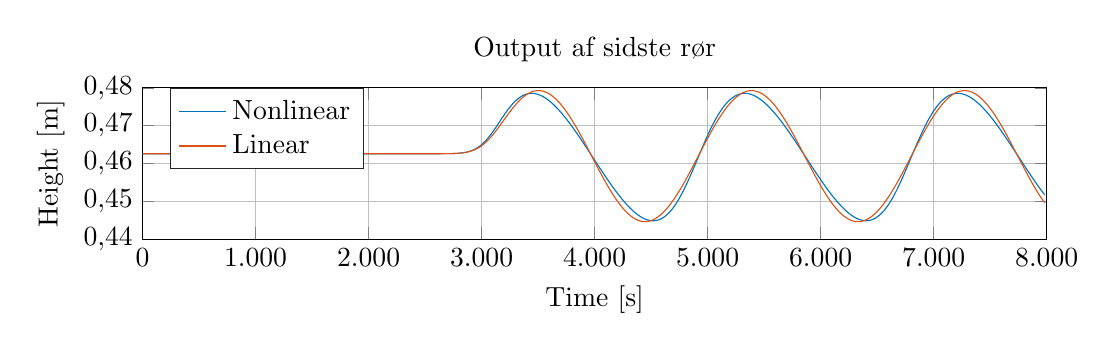
\begin{tikzpicture}

\begin{axis}[%
/pgf/number format/1000 sep={.},/pgf/number format/use comma,
width=4.521in,
height=.7566in,
at={(0.758in,0.481in)},
title ={Output af sidste rør},
scale only axis,
xmin=0,
xmax=8000,
xlabel={Time [s]},
xmajorgrids,
ymin=0.44,
ymax=0.48,
ylabel={Height [m]},
ymajorgrids,
axis background/.style={fill=white},
legend style={at={(0.03,0.73)},anchor=west},
legend style={legend cell align=left,align=left,draw=white!15!black}
]
\addplot [color=mycolor1,solid]
  table[row sep=crcr]{%
1	0.462595737606136\\
21	0.462595766861512\\
41	0.462595788438212\\
61	0.462595804181262\\
81	0.462595814989754\\
101	0.462595822807541\\
121	0.462595828630341\\
141	0.462595831905002\\
161	0.46259583412694\\
181	0.462595835844178\\
201	0.46259583699152\\
221	0.462595837729411\\
241	0.462595838185094\\
261	0.462595838461284\\
281	0.462595838623183\\
301	0.462595838711559\\
321	0.462595838750496\\
341	0.462595838752465\\
361	0.462595838721921\\
381	0.4625958386577\\
401	0.462595838554844\\
421	0.462595838406286\\
441	0.462595838204706\\
461	0.462595837944688\\
481	0.462595837625152\\
501	0.462595837251777\\
521	0.462595836838943\\
541	0.462595836410552\\
561	0.462595835999083\\
581	0.462595835642428\\
601	0.462595835378522\\
621	0.462595835238424\\
641	0.462595835239241\\
661	0.462595835378802\\
681	0.46259583563429\\
701	0.462595835965956\\
721	0.462595836326009\\
741	0.46259583667134\\
761	0.4625958369772\\
781	0.4625958372469\\
801	0.462595837510601\\
821	0.462595837811341\\
841	0.462595838185321\\
861	0.462595838646099\\
881	0.462595839178928\\
901	0.462595839745095\\
921	0.46259584029132\\
941	0.462595840759923\\
961	0.462595841098575\\
981	0.462595841269344\\
1001	0.462595841255849\\
1021	0.462595841066583\\
1041	0.462595840733295\\
1061	0.462595840304786\\
1081	0.462595839837555\\
1101	0.462595839385396\\
1121	0.462595838990585\\
1141	0.46259583867887\\
1161	0.462595838458964\\
1181	0.462595838325511\\
1201	0.462595838263768\\
1221	0.462595838254625\\
1241	0.46259583827901\\
1261	0.462595838320843\\
1281	0.462595838368157\\
1301	0.462595838412909\\
1321	0.462595838450395\\
1341	0.462595838478712\\
1361	0.462595838498255\\
1381	0.462595838511093\\
1401	0.462595838520255\\
1421	0.462595838528997\\
1441	0.46259583854018\\
1461	0.462595838555826\\
1481	0.462595838576902\\
1501	0.462595838603326\\
1521	0.462595838634151\\
1541	0.462595838667868\\
1561	0.462595838702734\\
1581	0.462595838737085\\
1601	0.462595838769557\\
1621	0.462595838799224\\
1641	0.462595838825622\\
1661	0.462595838848708\\
1681	0.462595838868759\\
1701	0.462595838886248\\
1721	0.462595838901721\\
1741	0.462595838915697\\
1761	0.462595838928591\\
1781	0.462595838940672\\
1801	0.462595838952052\\
1821	0.462595838962696\\
1841	0.462595838972448\\
1861	0.462595838981077\\
1881	0.462595838988318\\
1901	0.462595838993921\\
1921	0.462595838997697\\
1941	0.462595838999561\\
1961	0.462595838999575\\
1981	0.46259583899799\\
2001	0.462595838995287\\
2021	0.462595838992234\\
2041	0.462595838989955\\
2061	0.462595838990038\\
2081	0.462595838994679\\
2101	0.462595839006901\\
2121	0.462595839030852\\
2141	0.462595839072207\\
2161	0.46259583913876\\
2181	0.462595839241085\\
2201	0.462595839393452\\
2221	0.46259583961568\\
2241	0.462595839932888\\
2261	0.462595840379253\\
2281	0.462595841008547\\
2301	0.462595841858163\\
2321	0.462595843019391\\
2341	0.462595845638368\\
2361	0.4625958503106\\
2381	0.462595859125907\\
2401	0.462595874224808\\
2421	0.462595900568092\\
2441	0.46259594452641\\
2461	0.462596017209568\\
2481	0.462596133918965\\
2501	0.46259631785381\\
2521	0.462596599644938\\
2541	0.462597020085767\\
2561	0.462597629452957\\
2581	0.462598485211012\\
2601	0.462599653291652\\
2621	0.462601211614999\\
2641	0.462603270910744\\
2661	0.462606029337465\\
2681	0.462609870904031\\
2701	0.462615503569196\\
2721	0.462624112607928\\
2741	0.46263746573282\\
2761	0.462657927696744\\
2781	0.462688381305962\\
2801	0.462732126967519\\
2821	0.462792864345572\\
2841	0.462874800132007\\
2861	0.462982841012624\\
2881	0.463122751733321\\
2901	0.463301164887028\\
2921	0.463525383693851\\
2941	0.46380298787616\\
2961	0.464141275319514\\
2981	0.464546603824099\\
3001	0.465023723738187\\
3021	0.465575183944166\\
3041	0.466200875608223\\
3061	0.46689772826717\\
3081	0.467659571541626\\
3101	0.468477192712524\\
3121	0.469338619310273\\
3141	0.470229627253143\\
3161	0.471134437404302\\
3181	0.472036545221497\\
3201	0.472919622001497\\
3221	0.473768403009473\\
3241	0.474569438513391\\
3261	0.475311578027022\\
3281	0.475986128991952\\
3301	0.476586746354644\\
3321	0.477109177892581\\
3341	0.477550972074841\\
3361	0.477911178826543\\
3381	0.478190045081274\\
3401	0.478388723973582\\
3421	0.478509035502311\\
3441	0.478553294684254\\
3461	0.478524182145815\\
3481	0.478424623537686\\
3501	0.478257655473047\\
3521	0.478026314785805\\
3541	0.477733602173121\\
3561	0.47738254089049\\
3581	0.476976268333965\\
3601	0.476518060397594\\
3621	0.476011245130712\\
3641	0.47545904309026\\
3661	0.474864444741386\\
3681	0.474230207689763\\
3701	0.473558971311616\\
3721	0.472853408563272\\
3741	0.472116313052822\\
3761	0.471350571701492\\
3781	0.470559055223807\\
3801	0.469744502902326\\
3821	0.46890945975873\\
3841	0.468056279308506\\
3861	0.467187177240587\\
3881	0.466304314240948\\
3901	0.465409881535387\\
3921	0.464506158709552\\
3941	0.463595522263966\\
3961	0.462680405309402\\
3981	0.461763228435224\\
4001	0.460846328385924\\
4021	0.459931908983245\\
4041	0.459022034624202\\
4061	0.458118676734636\\
4081	0.457223800806582\\
4101	0.456339455804367\\
4121	0.455467824654186\\
4141	0.454611226317651\\
4161	0.453772100251186\\
4181	0.452953008380687\\
4201	0.452156648696482\\
4221	0.451385836185714\\
4241	0.450643426029038\\
4261	0.449932219537888\\
4281	0.449254929113725\\
4301	0.448614234014938\\
4321	0.448012878569118\\
4341	0.447453739908417\\
4361	0.446939839558729\\
4381	0.44647434512201\\
4401	0.446060595554607\\
4421	0.445702133914107\\
4441	0.445402706742644\\
4461	0.445166217376767\\
4481	0.444996657184716\\
4501	0.444898049706583\\
4521	0.444874383117409\\
4541	0.44492951658114\\
4561	0.445067050035481\\
4581	0.445290221202826\\
4601	0.445601871076422\\
4621	0.446004444523707\\
4641	0.446499957370417\\
4661	0.447089881838418\\
4681	0.447774969484852\\
4701	0.448555042272362\\
4721	0.449428783250223\\
4741	0.450393554823214\\
4761	0.45144526123565\\
4781	0.452578251837083\\
4801	0.453785262092848\\
4821	0.455057437346058\\
4841	0.456384522015529\\
4861	0.457755226755352\\
4881	0.459157658479834\\
4901	0.460579627094341\\
4921	0.462008752073201\\
4941	0.463432475906272\\
4961	0.464838171688495\\
4981	0.466213456263541\\
5001	0.467546667482304\\
5021	0.468827352513423\\
5041	0.470046586556222\\
5061	0.471197030174627\\
5081	0.472272770363773\\
5101	0.47326907833629\\
5121	0.474182212148699\\
5141	0.475009326281446\\
5161	0.475748486206027\\
5181	0.476398737917896\\
5201	0.476960143226998\\
5221	0.477433691431886\\
5241	0.477821069930187\\
5261	0.478124357961283\\
5281	0.478345765912584\\
5301	0.478487512168895\\
5321	0.478551852779087\\
5341	0.478541225105437\\
5361	0.478458394214516\\
5381	0.478306501319248\\
5401	0.478088959216268\\
5421	0.477809253818152\\
5441	0.477470786118439\\
5461	0.477076832102931\\
5481	0.47663058647073\\
5501	0.476135203510236\\
5521	0.475593780336078\\
5541	0.475009322157177\\
5561	0.474384750282148\\
5581	0.473722950736162\\
5601	0.473026799430022\\
5621	0.472299112843751\\
5641	0.471542551269154\\
5661	0.470759559127656\\
5681	0.469952405277727\\
5701	0.469123311086455\\
5721	0.46827459196725\\
5741	0.467408727973271\\
5761	0.466528318390822\\
5781	0.465635944291262\\
5801	0.464734028972795\\
5821	0.463824799057408\\
5841	0.462910378851767\\
5861	0.461992942586901\\
5881	0.46107480193166\\
5901	0.460158366463992\\
5921	0.459246018746161\\
5941	0.458339996203401\\
5961	0.457442349924919\\
5981	0.456555007564153\\
6001	0.455679931876339\\
6021	0.454819317892116\\
6041	0.453975716454362\\
6061	0.453151976708548\\
6081	0.452351008301765\\
6101	0.451575506849199\\
6121	0.45082783219231\\
6141	0.45011012604789\\
6161	0.44942459097568\\
6181	0.448773759457978\\
6201	0.448160613471587\\
6221	0.447588521960639\\
6241	0.447061063222956\\
6261	0.446581841206566\\
6281	0.446154386327256\\
6301	0.445782158282598\\
6321	0.445468610966842\\
6341	0.445217263297646\\
6361	0.445031741841928\\
6381	0.444915805522321\\
6401	0.444873351165655\\
6421	0.444908375095223\\
6441	0.445024827615758\\
6461	0.445226374670698\\
6481	0.44551615481219\\
6501	0.445896648950466\\
6521	0.446369693538927\\
6541	0.446936551429178\\
6561	0.447597931288157\\
6581	0.448353893073814\\
6601	0.449203647859668\\
6621	0.450145285496265\\
6641	0.451175466306077\\
6661	0.452289145414588\\
6681	0.453479432844087\\
6701	0.454737664462013\\
6721	0.456053668294621\\
6741	0.457416125332722\\
6761	0.458812927152067\\
6781	0.460231491336431\\
6801	0.46165905732883\\
6821	0.463082994401577\\
6841	0.464491098548183\\
6861	0.465871807792967\\
6881	0.467214296420706\\
6901	0.468508496672756\\
6921	0.469745148426169\\
6941	0.470915920459634\\
6961	0.472013588267787\\
6981	0.473032219475206\\
7001	0.473967322860057\\
7021	0.47481590339856\\
7041	0.475576347428661\\
7061	0.476248121577524\\
7081	0.476831397634691\\
7101	0.477326787330237\\
7121	0.477735296963816\\
7141	0.478058431459727\\
7161	0.478298287415192\\
7181	0.478457505420165\\
7201	0.478539068078455\\
7221	0.478546037683092\\
7241	0.478481356255522\\
7261	0.478347811075521\\
7281	0.47814814757116\\
7301	0.477885233336003\\
7321	0.477562154680077\\
7341	0.47718219234894\\
7361	0.476748713890495\\
7381	0.476265061745663\\
7401	0.475734478814768\\
7421	0.475160074919235\\
7441	0.474544828462544\\
7461	0.473891618610476\\
7481	0.473203272704271\\
7501	0.472482591551528\\
7521	0.47173231978675\\
7541	0.470955075285571\\
7561	0.470153299337239\\
7581	0.469329283635555\\
7601	0.468485269260669\\
7621	0.46762355399642\\
7641	0.46674654299248\\
7661	0.465856729240419\\
7681	0.464956638572598\\
7701	0.464048776136871\\
7721	0.46313558283631\\
7741	0.462219395731453\\
7761	0.461302419061183\\
7781	0.460386724760111\\
7801	0.459474291527016\\
7821	0.458567071551398\\
7841	0.457667064714051\\
7861	0.456776382674666\\
7881	0.4558972891119\\
7901	0.455032205739806\\
7921	0.454183683091857\\
7941	0.453354349456739\\
7961	0.452546859370056\\
7981	0.451763857819755\\
};
\addlegendentry{Nonlinear};

\addplot [color=mycolor2,solid]
  table[row sep=crcr]{%
1	0.462595737606136\\
21	0.462595737606136\\
41	0.462595737606136\\
61	0.462595737606136\\
81	0.462595737606136\\
101	0.462595737606136\\
121	0.462595737606136\\
141	0.462595737606136\\
161	0.462595737606136\\
181	0.462595737606136\\
201	0.462595737606136\\
221	0.462595737606136\\
241	0.462595737606136\\
261	0.462595737606136\\
281	0.462595737606136\\
301	0.462595737606136\\
321	0.462595737606136\\
341	0.462595737606136\\
361	0.462595737606136\\
381	0.462595737606136\\
401	0.462595737606136\\
421	0.462595737606136\\
441	0.462595737606136\\
461	0.462595737606136\\
481	0.462595737606136\\
501	0.462595737606136\\
521	0.462595737606136\\
541	0.462595737606136\\
561	0.462595737606136\\
581	0.462595737606136\\
601	0.462595737606136\\
621	0.462595737606136\\
641	0.462595737606136\\
661	0.462595737606136\\
681	0.462595737606136\\
701	0.462595737606136\\
721	0.462595737606136\\
741	0.462595737606136\\
761	0.462595737606136\\
781	0.462595737606136\\
801	0.462595737606136\\
821	0.462595737606136\\
841	0.462595737606136\\
861	0.462595737606136\\
881	0.462595737606136\\
901	0.462595737606136\\
921	0.462595737606136\\
941	0.462595737606136\\
961	0.462595737606136\\
981	0.462595737606136\\
1001	0.462595737606136\\
1021	0.462595737606136\\
1041	0.462595737606136\\
1061	0.462595737606136\\
1081	0.462595737606136\\
1101	0.462595737606136\\
1121	0.462595737606136\\
1141	0.462595737606136\\
1161	0.462595737606136\\
1181	0.462595737606136\\
1201	0.462595737606136\\
1221	0.462595737606136\\
1241	0.462595737606136\\
1261	0.462595737606136\\
1281	0.462595737606136\\
1301	0.462595737606136\\
1321	0.462595737606136\\
1341	0.462595737606136\\
1361	0.462595737606136\\
1381	0.462595737606136\\
1401	0.462595737606136\\
1421	0.462595737606136\\
1441	0.462595737606136\\
1461	0.462595737606136\\
1481	0.462595737606136\\
1501	0.462595737606136\\
1521	0.462595737606136\\
1541	0.462595737606136\\
1561	0.462595737606136\\
1581	0.462595737606136\\
1601	0.462595737606136\\
1621	0.462595737606136\\
1641	0.462595737606136\\
1661	0.462595737606136\\
1681	0.462595737606136\\
1701	0.462595737606136\\
1721	0.462595737606136\\
1741	0.462595737606136\\
1761	0.462595737606136\\
1781	0.462595737606136\\
1801	0.462595737606136\\
1821	0.462595737606136\\
1841	0.462595737606136\\
1861	0.462595737606136\\
1881	0.462595737606136\\
1901	0.462595737606136\\
1921	0.462595737606136\\
1941	0.462595737606136\\
1961	0.462595737606136\\
1981	0.462595737606136\\
2001	0.462595737606136\\
2021	0.462595737606136\\
2041	0.462595737606137\\
2061	0.462595737606138\\
2081	0.462595737606143\\
2101	0.462595737606155\\
2121	0.462595737606185\\
2141	0.46259573760626\\
2161	0.462595737606442\\
2181	0.462595737606881\\
2201	0.462595737607915\\
2221	0.462595737610311\\
2241	0.462595737615764\\
2261	0.462595737627956\\
2281	0.462595737654733\\
2301	0.462595737712507\\
2321	0.462595737834964\\
2341	0.462595738089961\\
2361	0.462595738611605\\
2381	0.462595739659966\\
2401	0.462595741729845\\
2421	0.462595745744776\\
2441	0.462595753395649\\
2461	0.462595767718986\\
2481	0.46259579406274\\
2501	0.462595841663183\\
2521	0.462595926160661\\
2541	0.46259607351919\\
2561	0.462596325986425\\
2581	0.462596750931272\\
2601	0.462597453611603\\
2621	0.462598595125208\\
2641	0.462600416936953\\
2661	0.462603273389091\\
2681	0.462607673407811\\
2701	0.462614332126884\\
2721	0.462624232274053\\
2741	0.462638693851075\\
2761	0.462659448883477\\
2781	0.462688715905299\\
2801	0.462729266569813\\
2821	0.462784474648894\\
2841	0.462858336113408\\
2861	0.462955448443918\\
2881	0.463080938255977\\
2901	0.463240329068703\\
2921	0.463439345704039\\
2941	0.463683658163351\\
2961	0.463978575310206\\
2981	0.464328706373438\\
3001	0.46473761501669\\
3021	0.465207495286579\\
3041	0.465738900112641\\
3061	0.466330550555491\\
3081	0.466979247640297\\
3101	0.467679898990943\\
3121	0.468425660825992\\
3141	0.469208183838434\\
3161	0.470017940829825\\
3181	0.470844606270707\\
3201	0.471677454272659\\
3221	0.472505742144354\\
3241	0.473319051383251\\
3261	0.474107565612145\\
3281	0.474862274193669\\
3301	0.475575099532513\\
3321	0.476238954078418\\
3341	0.476847738850598\\
3361	0.47739629850329\\
3381	0.477880348625895\\
3401	0.478296389589548\\
3421	0.47864161850588\\
3441	0.478913847491583\\
3461	0.479111433077405\\
3481	0.479233218721608\\
3501	0.479278490232898\\
3521	0.479246942531599\\
3541	0.479138655495855\\
3561	0.478954076489315\\
3581	0.478694007363406\\
3601	0.478359594104554\\
3621	0.47795231772777\\
3641	0.477473985421703\\
3661	0.476926721285119\\
3681	0.476312956249171\\
3701	0.475635416959559\\
3721	0.474897113512448\\
3741	0.474101326013728\\
3761	0.473251589977429\\
3781	0.472351680606591\\
3801	0.47140559601645\\
3821	0.470417539470096\\
3841	0.46939190070374\\
3861	0.468333236423857\\
3881	0.467246250062632\\
3901	0.46613577088155\\
3921	0.46500673251596\\
3941	0.463864151055931\\
3961	0.462713102760771\\
3981	0.461558701506231\\
4001	0.460406076064587\\
4021	0.459260347318534\\
4041	0.45812660551014\\
4061	0.45700988762592\\
4081	0.455915155018524\\
4101	0.454847271364446\\
4121	0.453810981055686\\
4141	0.452810888121376\\
4161	0.451851435773001\\
4181	0.450936886664109\\
4201	0.450071303952199\\
4221	0.44925853324693\\
4241	0.448502185524851\\
4261	0.447805621086561\\
4281	0.44717193462757\\
4301	0.446603941489189\\
4321	0.446104165150538\\
4341	0.445674826017232\\
4361	0.445317831556572\\
4381	0.445034767823046\\
4401	0.444826892411812\\
4421	0.444695128871457\\
4441	0.444640062600852\\
4461	0.444661938248348\\
4481	0.444760658624848\\
4501	0.444935785135602\\
4521	0.445186539728794\\
4541	0.445511808352268\\
4561	0.445910145903041\\
4581	0.446379782647601\\
4601	0.446918632084476\\
4621	0.447524300214145\\
4641	0.448194096175091\\
4661	0.448925044198757\\
4681	0.449713896830289\\
4701	0.450557149356322\\
4721	0.451451055375714\\
4741	0.452391643444058\\
4761	0.453374734718002\\
4781	0.454395961521012\\
4801	0.45545078674808\\
4821	0.456534524023167\\
4841	0.457642358519826\\
4861	0.458769368352508\\
4881	0.459910546443511\\
4901	0.461060822768411\\
4921	0.462215086881164\\
4941	0.46336821061879\\
4961	0.464515070884764\\
4981	0.465650572409904\\
5001	0.466769670389626\\
5021	0.467867392896996\\
5041	0.468938862971997\\
5061	0.469979320288883\\
5081	0.470984142305344\\
5101	0.471948864799536\\
5121	0.472869201703713\\
5141	0.473741064146368\\
5161	0.474560578618265\\
5181	0.475324104181655\\
5201	0.476028248646237\\
5221	0.476669883639971\\
5241	0.477246158507807\\
5261	0.477754512976569\\
5281	0.478192688529737\\
5301	0.478558738441577\\
5321	0.478851036426055\\
5341	0.479068283862095\\
5361	0.479209515563092\\
5381	0.479274104065045\\
5401	0.479261762414245\\
5421	0.479172545442164\\
5441	0.479006849521838\\
5461	0.478765410806871\\
5481	0.478449301960847\\
5501	0.478059927391703\\
5521	0.47759901701223\\
5541	0.477068618554415\\
5561	0.476471088471782\\
5581	0.475809081470146\\
5601	0.475085538713283\\
5621	0.474303674755941\\
5641	0.473466963262213\\
5661	0.472579121572749\\
5681	0.471644094189362\\
5701	0.470666035250401\\
5721	0.469649290074747\\
5741	0.468598375856442\\
5761	0.4675179615957\\
5781	0.466412847355485\\
5801	0.465287942935794\\
5821	0.464148246060404\\
5841	0.462998820172995\\
5861	0.461844771941289\\
5881	0.460691228569151\\
5901	0.459543315017457\\
5921	0.458406131234925\\
5941	0.457284729500069\\
5961	0.456184091974945\\
5981	0.455109108570406\\
6001	0.454064555221213\\
6021	0.453055072667523\\
6041	0.452085145837008\\
6061	0.451159083919233\\
6081	0.450281001220785\\
6101	0.449454798886248\\
6121	0.448684147566193\\
6141	0.447972471109226\\
6161	0.447322931350511\\
6181	0.446738414064377\\
6201	0.446221516143404\\
6221	0.44577453406095\\
6241	0.445399453668385\\
6261	0.44509794137235\\
6281	0.444871336731251\\
6301	0.44472064650387\\
6321	0.444646540176539\\
6341	0.444649346988744\\
6361	0.444729054470383\\
6381	0.44488530849717\\
6401	0.445117414863933\\
6421	0.445424342368832\\
6441	0.445804727394777\\
6461	0.446256879967709\\
6481	0.446778791264812\\
6501	0.447368142539305\\
6521	0.448022315422174\\
6541	0.448738403555052\\
6561	0.449513225502585\\
6581	0.450343338886913\\
6601	0.451225055681454\\
6621	0.452154458596072\\
6641	0.453127418480799\\
6661	0.454139612670824\\
6681	0.45518654419122\\
6701	0.456263561736095\\
6721	0.457365880333411\\
6741	0.45848860260365\\
6761	0.459626740517885\\
6781	0.460775237558584\\
6801	0.461928991184708\\
6821	0.463082875501263\\
6841	0.464231764032626\\
6861	0.46537055249844\\
6881	0.466494181490907\\
6901	0.467597658952714\\
6921	0.468676082355742\\
6941	0.469724660482008\\
6961	0.470738734710082\\
6981	0.471713799712407\\
7001	0.472645523471557\\
7021	0.473529766526521\\
7041	0.474362600363495\\
7061	0.475140324869477\\
7081	0.47585948477112\\
7101	0.476516884985823\\
7121	0.477109604816833\\
7141	0.477635010929317\\
7161	0.478090769049734\\
7181	0.478474854336547\\
7201	0.478785560376182\\
7221	0.479021506764281\\
7241	0.479181645238563\\
7261	0.479265264336037\\
7281	0.479271992553897\\
7301	0.479201800000023\\
7321	0.479054998525797\\
7341	0.478832240340602\\
7361	0.478534515114191\\
7381	0.478163145579783\\
7401	0.477719781657424\\
7421	0.477206393123726\\
7441	0.476625260860548\\
7461	0.475978966721493\\
7481	0.475270382061256\\
7501	0.474502654978772\\
7521	0.473679196330847\\
7541	0.472803664578406\\
7561	0.471879949532692\\
7581	0.470912155073615\\
7601	0.46990458091704\\
7621	0.468861703512017\\
7641	0.467788156152819\\
7661	0.466688708394148\\
7681	0.465568244860965\\
7701	0.464431743547083\\
7721	0.463284253698947\\
7741	0.462130873382844\\
7761	0.460976726835226\\
7781	0.459826941696755\\
7801	0.458686626231234\\
7821	0.457560846630612\\
7841	0.456454604506922\\
7861	0.455372814671118\\
7881	0.454320283297567\\
7901	0.453301686571179\\
7921	0.452321549912062\\
7941	0.451384227869991\\
7961	0.450493884778019\\
7981	0.449654476251187\\
};
\addlegendentry{Linear};

\end{axis}
\end{tikzpicture}%
\caption{Comparison of the nonlinear and linear model at the last pipe in the setup.}
\label{fig:linear_nonlinear_comparison_last_pipe}
\end{figure}

A small difference can be seen at the peaks of the two graphs. The nonlinear model starts to rise faster and falls slower than the linear model. However, it can be seen that the two model crosses the operating point at each period and they are similar in phase and amplitude. The linear model, is therefore deemed to be an acceptable linearized model of the nonlinear system for small perturbations. It will therefore be used in the next section in the design of MPC. 